\documentclass[]{article}
\usepackage{lmodern}
\usepackage{amssymb,amsmath}
\usepackage{ifxetex,ifluatex}
\usepackage{fixltx2e} % provides \textsubscript
\ifnum 0\ifxetex 1\fi\ifluatex 1\fi=0 % if pdftex
  \usepackage[T1]{fontenc}
  \usepackage[utf8]{inputenc}
\else % if luatex or xelatex
  \ifxetex
    \usepackage{mathspec}
  \else
    \usepackage{fontspec}
  \fi
  \defaultfontfeatures{Ligatures=TeX,Scale=MatchLowercase}
\fi
% use upquote if available, for straight quotes in verbatim environments
\IfFileExists{upquote.sty}{\usepackage{upquote}}{}
% use microtype if available
\IfFileExists{microtype.sty}{%
\usepackage{microtype}
\UseMicrotypeSet[protrusion]{basicmath} % disable protrusion for tt fonts
}{}
\usepackage[margin=1in]{geometry}
\usepackage{hyperref}
\hypersetup{unicode=true,
            pdftitle={DDSAnalytics\_Case\_Study},
            pdfauthor={The Miner League - Brandon Croom, Sandesh Ojha, Sangrae Cho},
            pdfborder={0 0 0},
            breaklinks=true}
\urlstyle{same}  % don't use monospace font for urls
\usepackage{color}
\usepackage{fancyvrb}
\newcommand{\VerbBar}{|}
\newcommand{\VERB}{\Verb[commandchars=\\\{\}]}
\DefineVerbatimEnvironment{Highlighting}{Verbatim}{commandchars=\\\{\}}
% Add ',fontsize=\small' for more characters per line
\usepackage{framed}
\definecolor{shadecolor}{RGB}{248,248,248}
\newenvironment{Shaded}{\begin{snugshade}}{\end{snugshade}}
\newcommand{\KeywordTok}[1]{\textcolor[rgb]{0.13,0.29,0.53}{\textbf{#1}}}
\newcommand{\DataTypeTok}[1]{\textcolor[rgb]{0.13,0.29,0.53}{#1}}
\newcommand{\DecValTok}[1]{\textcolor[rgb]{0.00,0.00,0.81}{#1}}
\newcommand{\BaseNTok}[1]{\textcolor[rgb]{0.00,0.00,0.81}{#1}}
\newcommand{\FloatTok}[1]{\textcolor[rgb]{0.00,0.00,0.81}{#1}}
\newcommand{\ConstantTok}[1]{\textcolor[rgb]{0.00,0.00,0.00}{#1}}
\newcommand{\CharTok}[1]{\textcolor[rgb]{0.31,0.60,0.02}{#1}}
\newcommand{\SpecialCharTok}[1]{\textcolor[rgb]{0.00,0.00,0.00}{#1}}
\newcommand{\StringTok}[1]{\textcolor[rgb]{0.31,0.60,0.02}{#1}}
\newcommand{\VerbatimStringTok}[1]{\textcolor[rgb]{0.31,0.60,0.02}{#1}}
\newcommand{\SpecialStringTok}[1]{\textcolor[rgb]{0.31,0.60,0.02}{#1}}
\newcommand{\ImportTok}[1]{#1}
\newcommand{\CommentTok}[1]{\textcolor[rgb]{0.56,0.35,0.01}{\textit{#1}}}
\newcommand{\DocumentationTok}[1]{\textcolor[rgb]{0.56,0.35,0.01}{\textbf{\textit{#1}}}}
\newcommand{\AnnotationTok}[1]{\textcolor[rgb]{0.56,0.35,0.01}{\textbf{\textit{#1}}}}
\newcommand{\CommentVarTok}[1]{\textcolor[rgb]{0.56,0.35,0.01}{\textbf{\textit{#1}}}}
\newcommand{\OtherTok}[1]{\textcolor[rgb]{0.56,0.35,0.01}{#1}}
\newcommand{\FunctionTok}[1]{\textcolor[rgb]{0.00,0.00,0.00}{#1}}
\newcommand{\VariableTok}[1]{\textcolor[rgb]{0.00,0.00,0.00}{#1}}
\newcommand{\ControlFlowTok}[1]{\textcolor[rgb]{0.13,0.29,0.53}{\textbf{#1}}}
\newcommand{\OperatorTok}[1]{\textcolor[rgb]{0.81,0.36,0.00}{\textbf{#1}}}
\newcommand{\BuiltInTok}[1]{#1}
\newcommand{\ExtensionTok}[1]{#1}
\newcommand{\PreprocessorTok}[1]{\textcolor[rgb]{0.56,0.35,0.01}{\textit{#1}}}
\newcommand{\AttributeTok}[1]{\textcolor[rgb]{0.77,0.63,0.00}{#1}}
\newcommand{\RegionMarkerTok}[1]{#1}
\newcommand{\InformationTok}[1]{\textcolor[rgb]{0.56,0.35,0.01}{\textbf{\textit{#1}}}}
\newcommand{\WarningTok}[1]{\textcolor[rgb]{0.56,0.35,0.01}{\textbf{\textit{#1}}}}
\newcommand{\AlertTok}[1]{\textcolor[rgb]{0.94,0.16,0.16}{#1}}
\newcommand{\ErrorTok}[1]{\textcolor[rgb]{0.64,0.00,0.00}{\textbf{#1}}}
\newcommand{\NormalTok}[1]{#1}
\usepackage{graphicx,grffile}
\makeatletter
\def\maxwidth{\ifdim\Gin@nat@width>\linewidth\linewidth\else\Gin@nat@width\fi}
\def\maxheight{\ifdim\Gin@nat@height>\textheight\textheight\else\Gin@nat@height\fi}
\makeatother
% Scale images if necessary, so that they will not overflow the page
% margins by default, and it is still possible to overwrite the defaults
% using explicit options in \includegraphics[width, height, ...]{}
\setkeys{Gin}{width=\maxwidth,height=\maxheight,keepaspectratio}
\IfFileExists{parskip.sty}{%
\usepackage{parskip}
}{% else
\setlength{\parindent}{0pt}
\setlength{\parskip}{6pt plus 2pt minus 1pt}
}
\setlength{\emergencystretch}{3em}  % prevent overfull lines
\providecommand{\tightlist}{%
  \setlength{\itemsep}{0pt}\setlength{\parskip}{0pt}}
\setcounter{secnumdepth}{0}
% Redefines (sub)paragraphs to behave more like sections
\ifx\paragraph\undefined\else
\let\oldparagraph\paragraph
\renewcommand{\paragraph}[1]{\oldparagraph{#1}\mbox{}}
\fi
\ifx\subparagraph\undefined\else
\let\oldsubparagraph\subparagraph
\renewcommand{\subparagraph}[1]{\oldsubparagraph{#1}\mbox{}}
\fi

%%% Use protect on footnotes to avoid problems with footnotes in titles
\let\rmarkdownfootnote\footnote%
\def\footnote{\protect\rmarkdownfootnote}

%%% Change title format to be more compact
\usepackage{titling}

% Create subtitle command for use in maketitle
\providecommand{\subtitle}[1]{
  \posttitle{
    \begin{center}\large#1\end{center}
    }
}

\setlength{\droptitle}{-2em}

  \title{DDSAnalytics\_Case\_Study}
    \pretitle{\vspace{\droptitle}\centering\huge}
  \posttitle{\par}
    \author{The Miner League - Brandon Croom, Sandesh Ojha, Sangrae Cho}
    \preauthor{\centering\large\emph}
  \postauthor{\par}
      \predate{\centering\large\emph}
  \postdate{\par}
    \date{August 2, 2019}


\begin{document}
\maketitle

\section{Problem Objective}\label{problem-objective}

The team has been asked by DDSAnalytics to use an existing data set in
order to predict employee turnover. The team has been asked to identify
at least three contributing factors to turn over. Additionally, the team
has been asked to provide any additional insight they may see coming
from the data.

\section{Setup Steps}\label{setup-steps}

\subsection{Initial Library Import and Data Loading
Setup}\label{initial-library-import-and-data-loading-setup}

\begin{Shaded}
\begin{Highlighting}[]
\CommentTok{#Install Packages that may be used. Suppress loading messages for cleaniliness}
\CommentTok{#NOTE: Install strings are encoded in the markup but commented out if a user needs to install}
\CommentTok{# - Install tidyverse for data cleaning, easy of use and base plotting. This includes ggplot dplyr, and tidyr}
\CommentTok{# - Install plyr for additional data cleaning items}
\CommentTok{# - Install corrplot for correlation plots}
\CommentTok{# - Install ggpubr for better graphic visual groupings}
\CommentTok{#install.packages("tidyverse")}
\CommentTok{#install.packages("plyr")}
\CommentTok{#install.packages("corrplot")}
\CommentTok{#install.packages("ggpubr")}
\CommentTok{#install.packages("RColorBrewer")}
\CommentTok{#install.packages("ggthemes")}
\KeywordTok{library}\NormalTok{(tidyverse)}
\KeywordTok{library}\NormalTok{(plyr)}
\KeywordTok{library}\NormalTok{(corrplot)}
\KeywordTok{library}\NormalTok{(ggpubr)}
\KeywordTok{library}\NormalTok{(RColorBrewer)}
\KeywordTok{library}\NormalTok{(ggthemes)}

\CommentTok{#Set Working directory and filepaths}
\NormalTok{workingDirFilePath =}\StringTok{ "C:}\CharTok{\textbackslash{}\textbackslash{}}\StringTok{Users}\CharTok{\textbackslash{}\textbackslash{}}\StringTok{croomb}\CharTok{\textbackslash{}\textbackslash{}}\StringTok{OneDrive - BAT}\CharTok{\textbackslash{}\textbackslash{}}\StringTok{Desktop}\CharTok{\textbackslash{}\textbackslash{}}\StringTok{Personal Training}\CharTok{\textbackslash{}\textbackslash{}}\StringTok{SMU}\CharTok{\textbackslash{}\textbackslash{}}\StringTok{DS 6306 - Doing Data Science}\CharTok{\textbackslash{}\textbackslash{}}\StringTok{DS6306-MinerLeague-CaseStudy2}\CharTok{\textbackslash{}\textbackslash{}}\StringTok{DS6306-MinerLeague-CaseStudy2}\CharTok{\textbackslash{}\textbackslash{}}\StringTok{Data}\CharTok{\textbackslash{}\textbackslash{}}\StringTok{"}

\NormalTok{sourceFile =}\StringTok{ "CaseStudy2-data-csv.csv"}

\KeywordTok{setwd}\NormalTok{(workingDirFilePath)}

\CommentTok{#Load data from the file. Ensure strings don't come in as factors}
\NormalTok{empDF_raw =}\StringTok{ }\KeywordTok{read.csv}\NormalTok{(sourceFile)}
\end{Highlighting}
\end{Shaded}

\subsection{Initial Data Checks}\label{initial-data-checks}

\textbf{check for general data structure }check for missing values

\begin{Shaded}
\begin{Highlighting}[]
\CommentTok{#Check on number of rows and variables}
\KeywordTok{dim}\NormalTok{(empDF_raw)}
\end{Highlighting}
\end{Shaded}

\begin{verbatim}
## [1] 1470   35
\end{verbatim}

\begin{Shaded}
\begin{Highlighting}[]
\CommentTok{#Get the names of the variables}
\KeywordTok{names}\NormalTok{(empDF_raw)}
\end{Highlighting}
\end{Shaded}

\begin{verbatim}
##  [1] "Age"                      "Attrition"               
##  [3] "BusinessTravel"           "DailyRate"               
##  [5] "Department"               "DistanceFromHome"        
##  [7] "Education"                "EducationField"          
##  [9] "EmployeeCount"            "EmployeeNumber"          
## [11] "EnvironmentSatisfaction"  "Gender"                  
## [13] "HourlyRate"               "JobInvolvement"          
## [15] "JobLevel"                 "JobRole"                 
## [17] "JobSatisfaction"          "MaritalStatus"           
## [19] "MonthlyIncome"            "MonthlyRate"             
## [21] "NumCompaniesWorked"       "Over18"                  
## [23] "OverTime"                 "PercentSalaryHike"       
## [25] "PerformanceRating"        "RelationshipSatisfaction"
## [27] "StandardHours"            "StockOptionLevel"        
## [29] "TotalWorkingYears"        "TrainingTimesLastYear"   
## [31] "WorkLifeBalance"          "YearsAtCompany"          
## [33] "YearsInCurrentRole"       "YearsSinceLastPromotion" 
## [35] "YearsWithCurrManager"
\end{verbatim}

\begin{Shaded}
\begin{Highlighting}[]
\CommentTok{#Perform a summary view of the data}
\KeywordTok{summary}\NormalTok{(empDF_raw)}
\end{Highlighting}
\end{Shaded}

\begin{verbatim}
##       Age        Attrition            BusinessTravel   DailyRate     
##  Min.   :18.00   No :1233   Non-Travel       : 150   Min.   : 102.0  
##  1st Qu.:30.00   Yes: 237   Travel_Frequently: 277   1st Qu.: 465.0  
##  Median :36.00              Travel_Rarely    :1043   Median : 802.0  
##  Mean   :36.92                                       Mean   : 802.5  
##  3rd Qu.:43.00                                       3rd Qu.:1157.0  
##  Max.   :60.00                                       Max.   :1499.0  
##                                                                      
##                   Department  DistanceFromHome   Education    
##  Human Resources       : 63   Min.   : 1.000   Min.   :1.000  
##  Research & Development:961   1st Qu.: 2.000   1st Qu.:2.000  
##  Sales                 :446   Median : 7.000   Median :3.000  
##                               Mean   : 9.193   Mean   :2.913  
##                               3rd Qu.:14.000   3rd Qu.:4.000  
##                               Max.   :29.000   Max.   :5.000  
##                                                               
##           EducationField EmployeeCount EmployeeNumber  
##  Human Resources : 27    Min.   :1     Min.   :   1.0  
##  Life Sciences   :606    1st Qu.:1     1st Qu.: 491.2  
##  Marketing       :159    Median :1     Median :1020.5  
##  Medical         :464    Mean   :1     Mean   :1024.9  
##  Other           : 82    3rd Qu.:1     3rd Qu.:1555.8  
##  Technical Degree:132    Max.   :1     Max.   :2068.0  
##                                                        
##  EnvironmentSatisfaction    Gender      HourlyRate     JobInvolvement
##  Min.   :1.000           Female:588   Min.   : 30.00   Min.   :1.00  
##  1st Qu.:2.000           Male  :882   1st Qu.: 48.00   1st Qu.:2.00  
##  Median :3.000                        Median : 66.00   Median :3.00  
##  Mean   :2.722                        Mean   : 65.89   Mean   :2.73  
##  3rd Qu.:4.000                        3rd Qu.: 83.75   3rd Qu.:3.00  
##  Max.   :4.000                        Max.   :100.00   Max.   :4.00  
##                                                                      
##     JobLevel                          JobRole    JobSatisfaction
##  Min.   :1.000   Sales Executive          :326   Min.   :1.000  
##  1st Qu.:1.000   Research Scientist       :292   1st Qu.:2.000  
##  Median :2.000   Laboratory Technician    :259   Median :3.000  
##  Mean   :2.064   Manufacturing Director   :145   Mean   :2.729  
##  3rd Qu.:3.000   Healthcare Representative:131   3rd Qu.:4.000  
##  Max.   :5.000   Manager                  :102   Max.   :4.000  
##                  (Other)                  :215                  
##   MaritalStatus MonthlyIncome    MonthlyRate    NumCompaniesWorked
##  Divorced:327   Min.   : 1009   Min.   : 2094   Min.   :0.000     
##  Married :673   1st Qu.: 2911   1st Qu.: 8047   1st Qu.:1.000     
##  Single  :470   Median : 4919   Median :14236   Median :2.000     
##                 Mean   : 6503   Mean   :14313   Mean   :2.693     
##                 3rd Qu.: 8379   3rd Qu.:20462   3rd Qu.:4.000     
##                 Max.   :19999   Max.   :26999   Max.   :9.000     
##                                                                   
##  Over18   OverTime   PercentSalaryHike PerformanceRating
##  Y:1470   No :1054   Min.   :11.00     Min.   :3.000    
##           Yes: 416   1st Qu.:12.00     1st Qu.:3.000    
##                      Median :14.00     Median :3.000    
##                      Mean   :15.21     Mean   :3.154    
##                      3rd Qu.:18.00     3rd Qu.:3.000    
##                      Max.   :25.00     Max.   :4.000    
##                                                         
##  RelationshipSatisfaction StandardHours StockOptionLevel TotalWorkingYears
##  Min.   :1.000            Min.   :80    Min.   :0.0000   Min.   : 0.00    
##  1st Qu.:2.000            1st Qu.:80    1st Qu.:0.0000   1st Qu.: 6.00    
##  Median :3.000            Median :80    Median :1.0000   Median :10.00    
##  Mean   :2.712            Mean   :80    Mean   :0.7939   Mean   :11.28    
##  3rd Qu.:4.000            3rd Qu.:80    3rd Qu.:1.0000   3rd Qu.:15.00    
##  Max.   :4.000            Max.   :80    Max.   :3.0000   Max.   :40.00    
##                                                                           
##  TrainingTimesLastYear WorkLifeBalance YearsAtCompany   YearsInCurrentRole
##  Min.   :0.000         Min.   :1.000   Min.   : 0.000   Min.   : 0.000    
##  1st Qu.:2.000         1st Qu.:2.000   1st Qu.: 3.000   1st Qu.: 2.000    
##  Median :3.000         Median :3.000   Median : 5.000   Median : 3.000    
##  Mean   :2.799         Mean   :2.761   Mean   : 7.008   Mean   : 4.229    
##  3rd Qu.:3.000         3rd Qu.:3.000   3rd Qu.: 9.000   3rd Qu.: 7.000    
##  Max.   :6.000         Max.   :4.000   Max.   :40.000   Max.   :18.000    
##                                                                           
##  YearsSinceLastPromotion YearsWithCurrManager
##  Min.   : 0.000          Min.   : 0.000      
##  1st Qu.: 0.000          1st Qu.: 2.000      
##  Median : 1.000          Median : 3.000      
##  Mean   : 2.188          Mean   : 4.123      
##  3rd Qu.: 3.000          3rd Qu.: 7.000      
##  Max.   :15.000          Max.   :17.000      
## 
\end{verbatim}

\begin{Shaded}
\begin{Highlighting}[]
\CommentTok{#Perform a check for any nulls in the data}
\KeywordTok{sum}\NormalTok{(}\KeywordTok{is.na}\NormalTok{(empDF_raw))}
\end{Highlighting}
\end{Shaded}

\begin{verbatim}
## [1] 0
\end{verbatim}

\begin{Shaded}
\begin{Highlighting}[]
\CommentTok{#Looks like there are no NA values in the data}
\end{Highlighting}
\end{Shaded}

\subsection{Data manipulation}\label{data-manipulation}

\begin{Shaded}
\begin{Highlighting}[]
\CommentTok{#Do some data manipulation to make things a bit easier on our EDA. We'll perform the following tasks resulting in a new data frame. This will allow us to get #back to the original data set should something go amiss}

\CommentTok{#There are a bunch of catgorical values that look to be off a Likert scale. The data has the value. Let's add in the descriptor associated with the value to #allow for making things a bit nicer. We'll turn these values in to factors to do this. For code readability we'll break each statement up}

\CommentTok{#mutate Education}
\NormalTok{empDF_raw =}\StringTok{ }\NormalTok{empDF_raw }\OperatorTok
\StringTok{  }\KeywordTok{mutate}\NormalTok{(}\DataTypeTok{Education =} \KeywordTok{as.factor}\NormalTok{(}\KeywordTok{if_else}\NormalTok{(Education }\OperatorTok{==}\StringTok{ }\DecValTok{1}\NormalTok{,}\StringTok{"Below College"}\NormalTok{, }\KeywordTok{if_else}\NormalTok{(Education }\OperatorTok{==}\StringTok{ }\DecValTok{2}\NormalTok{, }\StringTok{"College"}\NormalTok{, }\KeywordTok{if_else}\NormalTok{(Education }\OperatorTok{==}\StringTok{ }\DecValTok{3}\NormalTok{, }\StringTok{"Bachelor"}\NormalTok{, }\KeywordTok{if_else}\NormalTok{(Education }\OperatorTok{==}\StringTok{ }\DecValTok{4}\NormalTok{, }\StringTok{"Master"}\NormalTok{,}\StringTok{"Doctor"}\NormalTok{))))))}

\CommentTok{#mutate Environmental Satisfaction}
\NormalTok{empDF_raw =}\StringTok{ }\NormalTok{empDF_raw }\OperatorTok
\StringTok{         }\KeywordTok{mutate}\NormalTok{(}\DataTypeTok{EnvironmentSatisfaction =} \KeywordTok{as.factor}\NormalTok{(}\KeywordTok{if_else}\NormalTok{(EnvironmentSatisfaction }\OperatorTok{==}\StringTok{ }\DecValTok{1}\NormalTok{,}\StringTok{"Low"}\NormalTok{,}\KeywordTok{if_else}\NormalTok{(EnvironmentSatisfaction }\OperatorTok{==}\StringTok{ }\DecValTok{2}\NormalTok{, }\StringTok{"Medium"}\NormalTok{, }\KeywordTok{if_else}\NormalTok{(EnvironmentSatisfaction }\OperatorTok{==}\StringTok{ }\DecValTok{3}\NormalTok{, }\StringTok{"High"}\NormalTok{, }\StringTok{"Very High"}\NormalTok{)))))}

\CommentTok{#mutate Job Involvement}
\NormalTok{empDF_raw =}\StringTok{ }\NormalTok{empDF_raw }\OperatorTok\StringTok{ }\KeywordTok{mutate}\NormalTok{(}\DataTypeTok{JobInvolvement =} \KeywordTok{as.factor}\NormalTok{(}\KeywordTok{if_else}\NormalTok{(JobInvolvement }\OperatorTok{==}\StringTok{ }\DecValTok{1}\NormalTok{,}\StringTok{"Low"}\NormalTok{,}\KeywordTok{if_else}\NormalTok{(JobInvolvement }\OperatorTok{==}\StringTok{ }\DecValTok{2}\NormalTok{, }\StringTok{"Medium"}\NormalTok{,}\KeywordTok{if_else}\NormalTok{(JobInvolvement }\OperatorTok{==}\StringTok{ }\DecValTok{3}\NormalTok{, }\StringTok{"High"}\NormalTok{, }\StringTok{"Very High"}\NormalTok{)))))}
 
\CommentTok{#mutate Job Satisfaction}
\NormalTok{empDF_raw =}\StringTok{ }\NormalTok{empDF_raw }\OperatorTok\StringTok{ }\KeywordTok{mutate}\NormalTok{(}\DataTypeTok{JobSatisfaction =} \KeywordTok{as.factor}\NormalTok{(}\KeywordTok{if_else}\NormalTok{(JobSatisfaction }\OperatorTok{==}\StringTok{ }\DecValTok{1}\NormalTok{, }\StringTok{"Low"}\NormalTok{,}\KeywordTok{if_else}\NormalTok{(JobSatisfaction }\OperatorTok{==}\StringTok{ }\DecValTok{2}\NormalTok{, }\StringTok{"Medium"}\NormalTok{,}\KeywordTok{if_else}\NormalTok{(JobSatisfaction }\OperatorTok{==}\StringTok{ }\DecValTok{3}\NormalTok{, }\StringTok{"High"}\NormalTok{,}\StringTok{"Very High"}\NormalTok{)))))}
 
\CommentTok{#mutate Performance Rating}
\NormalTok{empDF_raw =}\StringTok{ }\NormalTok{empDF_raw }\OperatorTok\StringTok{ }\KeywordTok{mutate}\NormalTok{(}\DataTypeTok{PerformanceRating =} \KeywordTok{as.factor}\NormalTok{(}\KeywordTok{if_else}\NormalTok{(PerformanceRating }\OperatorTok{==}\StringTok{ }\DecValTok{1}\NormalTok{, }\StringTok{"Low"}\NormalTok{,}\KeywordTok{if_else}\NormalTok{(PerformanceRating }\OperatorTok{==}\StringTok{ }\DecValTok{2}\NormalTok{, }\StringTok{"Good"}\NormalTok{, }\KeywordTok{if_else}\NormalTok{(PerformanceRating }\OperatorTok{==}\StringTok{ }\DecValTok{3}\NormalTok{, }\StringTok{"Excellent"}\NormalTok{, }\StringTok{"Outstanding"}\NormalTok{)))))}

\CommentTok{#mutate Relationship Satisfaction}
\NormalTok{empDF_raw =}\StringTok{ }\NormalTok{empDF_raw }\OperatorTok\StringTok{ }\KeywordTok{mutate}\NormalTok{(}\DataTypeTok{RelationshipSatisfaction =} \KeywordTok{as.factor}\NormalTok{(}\KeywordTok{if_else}\NormalTok{(RelationshipSatisfaction }\OperatorTok{==}\StringTok{ }\DecValTok{1}\NormalTok{, }\StringTok{"Low"}\NormalTok{,}\KeywordTok{if_else}\NormalTok{(RelationshipSatisfaction }\OperatorTok{==}\StringTok{ }\DecValTok{2}\NormalTok{, }\StringTok{"Medium"}\NormalTok{, }\KeywordTok{if_else}\NormalTok{(RelationshipSatisfaction }\OperatorTok{==}\StringTok{ }\DecValTok{3}\NormalTok{, }\StringTok{"High"}\NormalTok{, }\StringTok{"Very High"}\NormalTok{)))))}

\CommentTok{#mutate Work Life Balance}
\NormalTok{empDF_raw =}\StringTok{ }\NormalTok{empDF_raw }\OperatorTok\StringTok{ }\KeywordTok{mutate}\NormalTok{(}\DataTypeTok{WorkLifeBalance =} \KeywordTok{as.factor}\NormalTok{(}\KeywordTok{if_else}\NormalTok{(WorkLifeBalance }\OperatorTok{==}\StringTok{ }\DecValTok{1}\NormalTok{, }\StringTok{"Bad"}\NormalTok{,}\KeywordTok{if_else}\NormalTok{(WorkLifeBalance }\OperatorTok{==}\StringTok{ }\DecValTok{2}\NormalTok{, }\StringTok{"Good"}\NormalTok{, }\KeywordTok{if_else}\NormalTok{(WorkLifeBalance }\OperatorTok{==}\StringTok{ }\DecValTok{3}\NormalTok{, }\StringTok{"Better"}\NormalTok{, }\StringTok{"Best"}\NormalTok{)))))}

\CommentTok{#mutate Job Level}
\NormalTok{empDF_raw =}\StringTok{ }\NormalTok{empDF_raw }\OperatorTok\StringTok{ }\KeywordTok{mutate}\NormalTok{(}\DataTypeTok{JobLevel =} \KeywordTok{as.factor}\NormalTok{(JobLevel))}

\CommentTok{#In looking at the summary data we can see that the following fields are "static" (e.g. have no variation). Let's remove them to ensure they don't get mixed in. }
\CommentTok{#Specifically:}
\CommentTok{# - Over18 - all values are "Y"}
\CommentTok{# - EmployeeCount - all values are 1}
\CommentTok{# - StandardHours - no variation all values are 80}
\CommentTok{# - EmployeeNumber - this is just a reference column}
\NormalTok{empDF =}\StringTok{ }\NormalTok{dplyr}\OperatorTok{::}\KeywordTok{select}\NormalTok{(empDF_raw, }\OperatorTok{-}\KeywordTok{c}\NormalTok{(}\StringTok{"Over18"}\NormalTok{,}\StringTok{"EmployeeCount"}\NormalTok{,}\StringTok{"StandardHours"}\NormalTok{,}\StringTok{"EmployeeNumber"}\NormalTok{))}

\CommentTok{#Check out structure to make sure the columns were removed}
\KeywordTok{str}\NormalTok{(empDF)}
\end{Highlighting}
\end{Shaded}

\begin{verbatim}
## 'data.frame':    1470 obs. of  31 variables:
##  $ Age                     : int  41 49 37 33 27 32 59 30 38 36 ...
##  $ Attrition               : Factor w/ 2 levels "No","Yes": 2 1 2 1 1 1 1 1 1 1 ...
##  $ BusinessTravel          : Factor w/ 3 levels "Non-Travel","Travel_Frequently",..: 3 2 3 2 3 2 3 3 2 3 ...
##  $ DailyRate               : int  1102 279 1373 1392 591 1005 1324 1358 216 1299 ...
##  $ Department              : Factor w/ 3 levels "Human Resources",..: 3 2 2 2 2 2 2 2 2 2 ...
##  $ DistanceFromHome        : int  1 8 2 3 2 2 3 24 23 27 ...
##  $ Education               : Factor w/ 5 levels "Bachelor","Below College",..: 3 2 3 5 2 3 1 2 1 1 ...
##  $ EducationField          : Factor w/ 6 levels "Human Resources",..: 2 2 5 2 4 2 4 2 2 4 ...
##  $ EnvironmentSatisfaction : Factor w/ 4 levels "High","Low","Medium",..: 3 1 4 4 2 4 1 4 4 1 ...
##  $ Gender                  : Factor w/ 2 levels "Female","Male": 1 2 2 1 2 2 1 2 2 2 ...
##  $ HourlyRate              : int  94 61 92 56 40 79 81 67 44 94 ...
##  $ JobInvolvement          : Factor w/ 4 levels "High","Low","Medium",..: 1 3 3 1 1 1 4 1 3 1 ...
##  $ JobLevel                : Factor w/ 5 levels "1","2","3","4",..: 2 2 1 1 1 1 1 1 3 2 ...
##  $ JobRole                 : Factor w/ 9 levels "Healthcare Representative",..: 8 7 3 7 3 3 3 3 5 1 ...
##  $ JobSatisfaction         : Factor w/ 4 levels "High","Low","Medium",..: 4 3 1 1 3 4 2 1 1 1 ...
##  $ MaritalStatus           : Factor w/ 3 levels "Divorced","Married",..: 3 2 3 2 2 3 2 1 3 2 ...
##  $ MonthlyIncome           : int  5993 5130 2090 2909 3468 3068 2670 2693 9526 5237 ...
##  $ MonthlyRate             : int  19479 24907 2396 23159 16632 11864 9964 13335 8787 16577 ...
##  $ NumCompaniesWorked      : int  8 1 6 1 9 0 4 1 0 6 ...
##  $ OverTime                : Factor w/ 2 levels "No","Yes": 2 1 2 2 1 1 2 1 1 1 ...
##  $ PercentSalaryHike       : int  11 23 15 11 12 13 20 22 21 13 ...
##  $ PerformanceRating       : Factor w/ 2 levels "Excellent","Outstanding": 1 2 1 1 1 1 2 2 2 1 ...
##  $ RelationshipSatisfaction: Factor w/ 4 levels "High","Low","Medium",..: 2 4 3 1 4 1 2 3 3 3 ...
##  $ StockOptionLevel        : int  0 1 0 0 1 0 3 1 0 2 ...
##  $ TotalWorkingYears       : int  8 10 7 8 6 8 12 1 10 17 ...
##  $ TrainingTimesLastYear   : int  0 3 3 3 3 2 3 2 2 3 ...
##  $ WorkLifeBalance         : Factor w/ 4 levels "Bad","Best","Better",..: 1 3 3 3 3 4 4 3 3 4 ...
##  $ YearsAtCompany          : int  6 10 0 8 2 7 1 1 9 7 ...
##  $ YearsInCurrentRole      : int  4 7 0 7 2 7 0 0 7 7 ...
##  $ YearsSinceLastPromotion : int  0 1 0 3 2 3 0 0 1 7 ...
##  $ YearsWithCurrManager    : int  5 7 0 0 2 6 0 0 8 7 ...
\end{verbatim}

\begin{center}\rule{0.5\linewidth}{\linethickness}\end{center}

\section{Univariate EDA}\label{univariate-eda}

Look at the data values individually without worrying about the
attrition variable. See if there are any interesting observations. Start
first with non-categorical (numeric) variables and then analyze
categorical variables.

\subsection{Non-Categorical Variables}\label{non-categorical-variables}

\subsubsection{Employee Demographics -
Basic}\label{employee-demographics---basic}

\begin{Shaded}
\begin{Highlighting}[]
\CommentTok{#Look at basic total employee demographics such as Age, Working Years, Companies worked for and Distance from Home}
\CommentTok{#Age breakdown}
\NormalTok{p1 =}\StringTok{ }\KeywordTok{ggplot}\NormalTok{(empDF) }\OperatorTok{+}\StringTok{ }\KeywordTok{geom_histogram}\NormalTok{(}\KeywordTok{aes}\NormalTok{(Age), }\DataTypeTok{binwidth=}\DecValTok{5}\NormalTok{, }\DataTypeTok{fill=}\StringTok{"green"}\NormalTok{, }\DataTypeTok{col=}\StringTok{"black"}\NormalTok{)}

\CommentTok{#Total Working Years}
\NormalTok{p2 =}\StringTok{ }\KeywordTok{ggplot}\NormalTok{(empDF) }\OperatorTok{+}\StringTok{ }\KeywordTok{geom_histogram}\NormalTok{(}\KeywordTok{aes}\NormalTok{(TotalWorkingYears),}\DataTypeTok{binwidth=}\DecValTok{5}\NormalTok{, }\DataTypeTok{fill=}\StringTok{"green"}\NormalTok{, }\DataTypeTok{col=}\StringTok{"black"}\NormalTok{)}

\CommentTok{#Number of Companies Worked}
\NormalTok{p3 =}\StringTok{ }\KeywordTok{ggplot}\NormalTok{(empDF) }\OperatorTok{+}\StringTok{ }\KeywordTok{geom_histogram}\NormalTok{(}\KeywordTok{aes}\NormalTok{(NumCompaniesWorked),}\DataTypeTok{binwidth=}\DecValTok{2}\NormalTok{, }\DataTypeTok{fill=}\StringTok{"green"}\NormalTok{, }\DataTypeTok{col=}\StringTok{"black"}\NormalTok{)}

\CommentTok{#Distance From Home}
\NormalTok{p4 =}\StringTok{ }\KeywordTok{ggplot}\NormalTok{(empDF) }\OperatorTok{+}\StringTok{ }\KeywordTok{geom_histogram}\NormalTok{(}\KeywordTok{aes}\NormalTok{(DistanceFromHome),}\DataTypeTok{binwidth=}\DecValTok{5}\NormalTok{, }\DataTypeTok{fill=}\StringTok{"green"}\NormalTok{, }\DataTypeTok{col=}\StringTok{"black"}\NormalTok{)}

\KeywordTok{ggarrange}\NormalTok{(p1,p2,p3,p4)}
\end{Highlighting}
\end{Shaded}

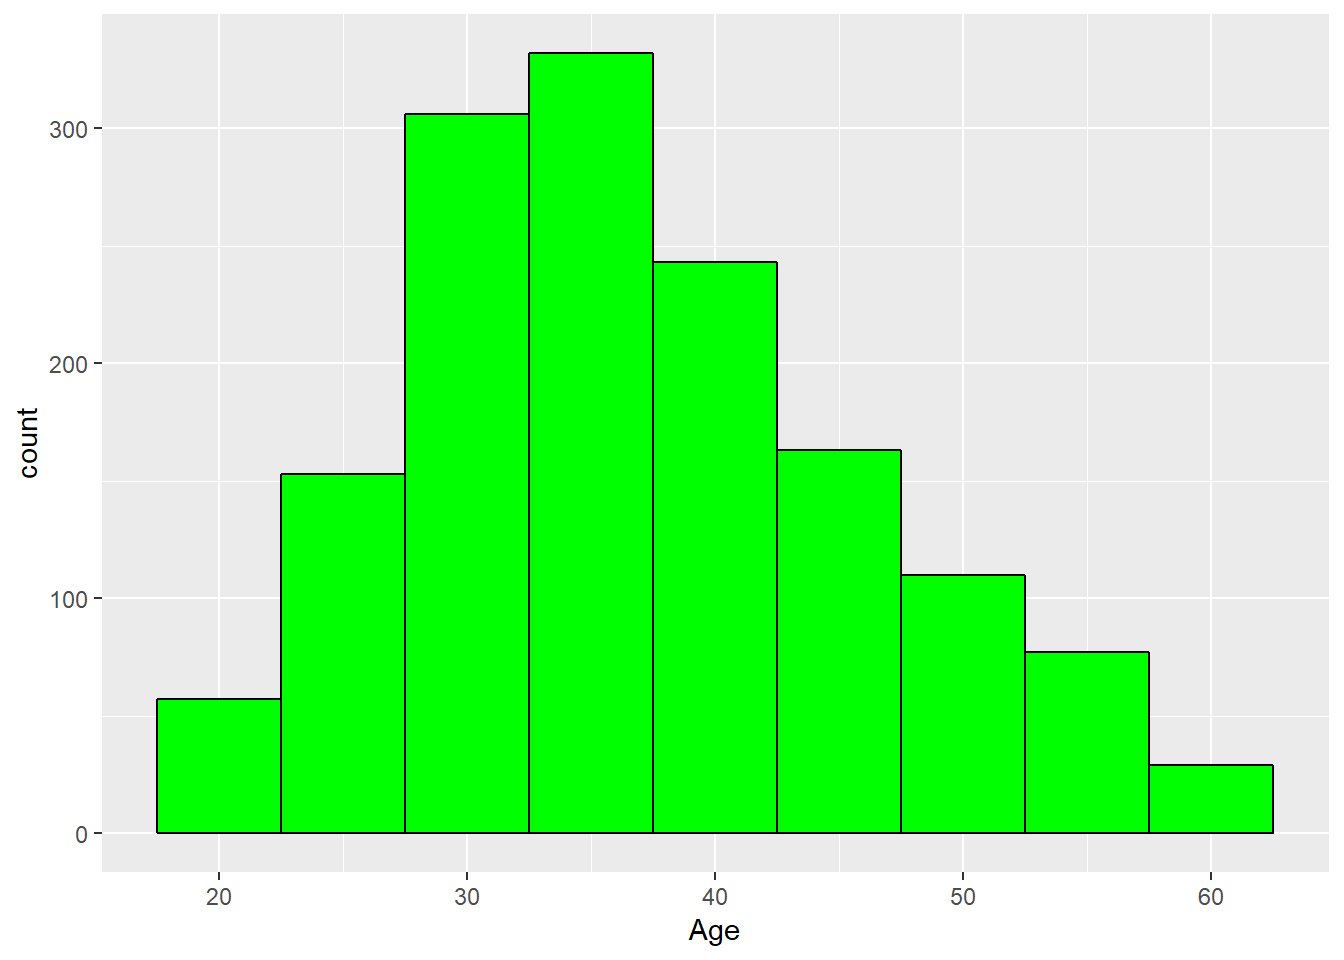
\includegraphics{DDSAnalytics_Case_Study_files/figure-latex/uni_non_cat_demo_basic-1.pdf}

\subsubsection{Observations}\label{observations}

\begin{itemize}
\tightlist
\item
  Age data looks to be normally distributed.
\item
  Total Working Years, Number of Companies Worked For, and Distance From
  Home are all right skewed. Transformation of this data may be
  necessary for further analysis
\end{itemize}

\subsubsection{Employee Demographics -
Financial}\label{employee-demographics---financial}

\begin{Shaded}
\begin{Highlighting}[]
\CommentTok{#Look at total employee financial demographics such as DailyRate, HourlyRate, MonthlyRate}

\CommentTok{#HourlyRate}
\NormalTok{p1 =}\StringTok{ }\KeywordTok{ggplot}\NormalTok{(empDF) }\OperatorTok{+}\StringTok{ }\KeywordTok{geom_histogram}\NormalTok{(}\KeywordTok{aes}\NormalTok{(HourlyRate), }\DataTypeTok{binwidth =} \DecValTok{5}\NormalTok{, }\DataTypeTok{fill=}\StringTok{"blue"}\NormalTok{, }\DataTypeTok{col=}\StringTok{"black"}\NormalTok{)}

\CommentTok{#DailyRate}
\NormalTok{p2 =}\StringTok{ }\KeywordTok{ggplot}\NormalTok{(empDF) }\OperatorTok{+}\StringTok{ }\KeywordTok{geom_histogram}\NormalTok{(}\KeywordTok{aes}\NormalTok{(DailyRate), }\DataTypeTok{binwidth =} \DecValTok{100}\NormalTok{, }\DataTypeTok{fill=}\StringTok{"blue"}\NormalTok{, }\DataTypeTok{col=}\StringTok{"black"}\NormalTok{)}

\CommentTok{#MonthlyRate}
\NormalTok{p3 =}\StringTok{ }\KeywordTok{ggplot}\NormalTok{(empDF) }\OperatorTok{+}\StringTok{ }\KeywordTok{geom_histogram}\NormalTok{(}\KeywordTok{aes}\NormalTok{(MonthlyRate), }\DataTypeTok{binwidth =} \DecValTok{1000}\NormalTok{, }\DataTypeTok{fill=}\StringTok{"blue"}\NormalTok{, }\DataTypeTok{col=}\StringTok{"black"}\NormalTok{)}

\KeywordTok{ggarrange}\NormalTok{(p1,p2,p3)}
\end{Highlighting}
\end{Shaded}

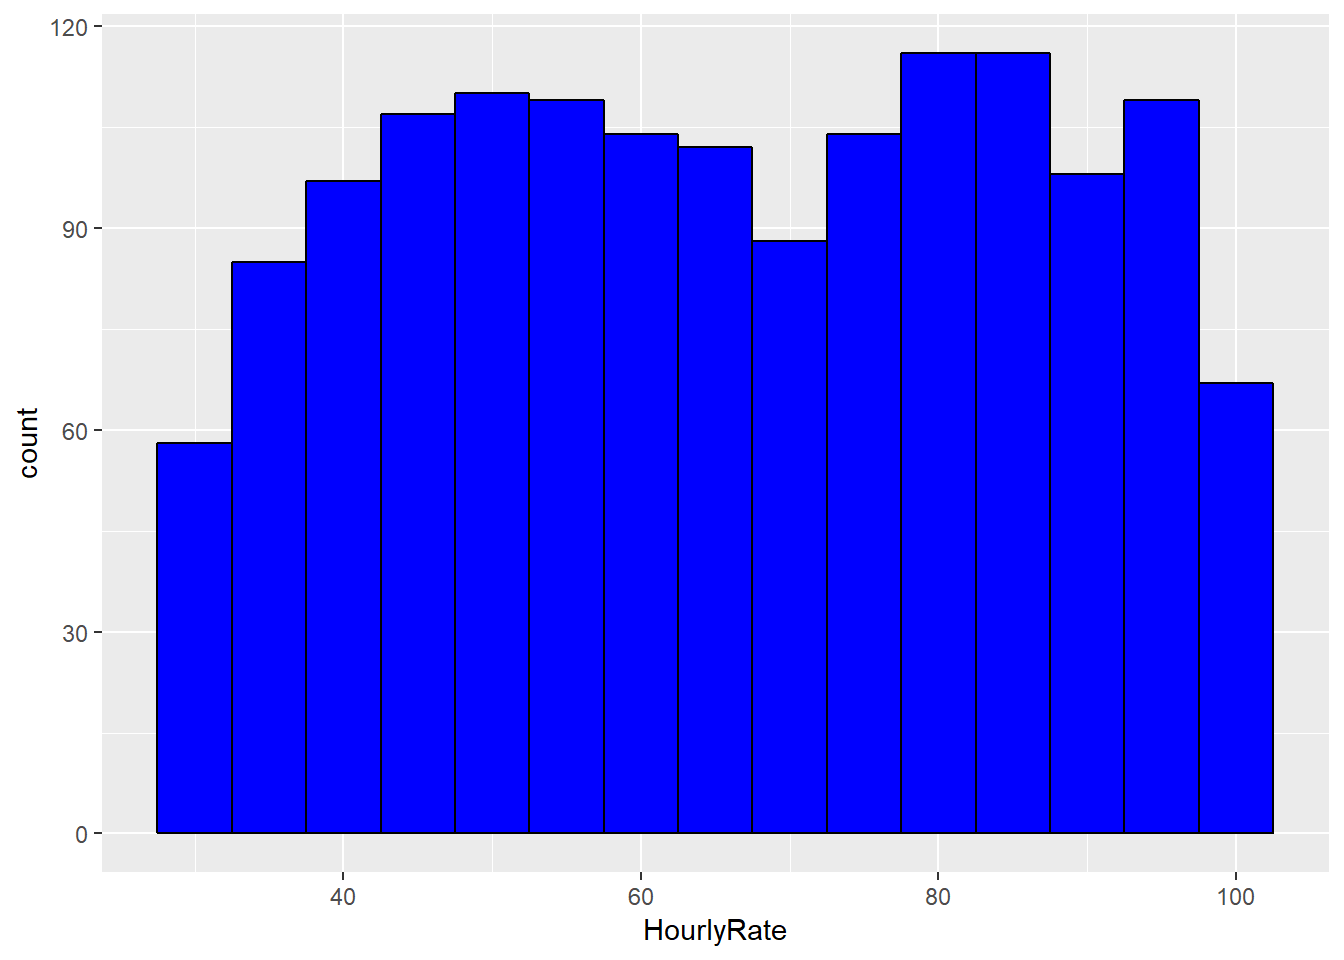
\includegraphics{DDSAnalytics_Case_Study_files/figure-latex/uni_non_cat_demo_financial-1.pdf}

\subsubsection{Observations}\label{observations-1}

\begin{itemize}
\tightlist
\item
  No patterns are observed in this data.
\end{itemize}

\subsubsection{Employee Demographics - Work
Environment}\label{employee-demographics---work-environment}

\begin{Shaded}
\begin{Highlighting}[]
\CommentTok{#Look at work environment dempgraphics such as income, years in current role,  time with current manager, years since last promotion}
\CommentTok{#training time, years at company}
\CommentTok{#Monthly Income}
\NormalTok{p1 =}\StringTok{ }\KeywordTok{ggplot}\NormalTok{(empDF) }\OperatorTok{+}\StringTok{ }\KeywordTok{geom_histogram}\NormalTok{(}\KeywordTok{aes}\NormalTok{(MonthlyIncome), }\DataTypeTok{binwidth =} \DecValTok{1000}\NormalTok{, }\DataTypeTok{fill =} \StringTok{"orange"}\NormalTok{,}\DataTypeTok{col =} \StringTok{"black"}\NormalTok{)}

\CommentTok{#Percent Salary Hike}
\NormalTok{p2 =}\StringTok{ }\KeywordTok{ggplot}\NormalTok{(empDF) }\OperatorTok{+}\StringTok{ }\KeywordTok{geom_histogram}\NormalTok{(}\KeywordTok{aes}\NormalTok{(PercentSalaryHike), }\DataTypeTok{binwidth =} \DecValTok{1}\NormalTok{, }\DataTypeTok{fill =} \StringTok{"orange"}\NormalTok{,}\DataTypeTok{col =} \StringTok{"black"}\NormalTok{)}

\CommentTok{#Years At Company}
\NormalTok{p3 =}\StringTok{ }\KeywordTok{ggplot}\NormalTok{(empDF) }\OperatorTok{+}\StringTok{ }\KeywordTok{geom_histogram}\NormalTok{(}\KeywordTok{aes}\NormalTok{(YearsAtCompany), }\DataTypeTok{binwidth =} \DecValTok{2}\NormalTok{, }\DataTypeTok{fill =} \StringTok{"orange"}\NormalTok{,}\DataTypeTok{col =} \StringTok{"black"}\NormalTok{)}

\CommentTok{#Years in Current Role}
\NormalTok{p4 =}\StringTok{ }\KeywordTok{ggplot}\NormalTok{(empDF) }\OperatorTok{+}\StringTok{ }\KeywordTok{geom_histogram}\NormalTok{(}\KeywordTok{aes}\NormalTok{(YearsInCurrentRole), }\DataTypeTok{binwidth =} \DecValTok{2}\NormalTok{, }\DataTypeTok{fill =} \StringTok{"orange"}\NormalTok{,}\DataTypeTok{col =} \StringTok{"black"}\NormalTok{)}

\CommentTok{#Years Since Last Promotion}
\NormalTok{p5 =}\StringTok{ }\KeywordTok{ggplot}\NormalTok{(empDF) }\OperatorTok{+}\StringTok{ }\KeywordTok{geom_histogram}\NormalTok{(}\KeywordTok{aes}\NormalTok{(YearsSinceLastPromotion), }\DataTypeTok{binwidth =} \DecValTok{2}\NormalTok{, }\DataTypeTok{fill =} \StringTok{"orange"}\NormalTok{,}\DataTypeTok{col =} \StringTok{"black"}\NormalTok{)}

\CommentTok{#Years with Current Manager}
\NormalTok{p6 =}\StringTok{ }\KeywordTok{ggplot}\NormalTok{(empDF) }\OperatorTok{+}\StringTok{ }\KeywordTok{geom_histogram}\NormalTok{(}\KeywordTok{aes}\NormalTok{(YearsWithCurrManager), }\DataTypeTok{binwidth =} \DecValTok{2}\NormalTok{, }\DataTypeTok{fill =} \StringTok{"orange"}\NormalTok{,}\DataTypeTok{col =} \StringTok{"black"}\NormalTok{)}

\KeywordTok{ggarrange}\NormalTok{(p1,p2,p3,p4,p5,p6)}
\end{Highlighting}
\end{Shaded}

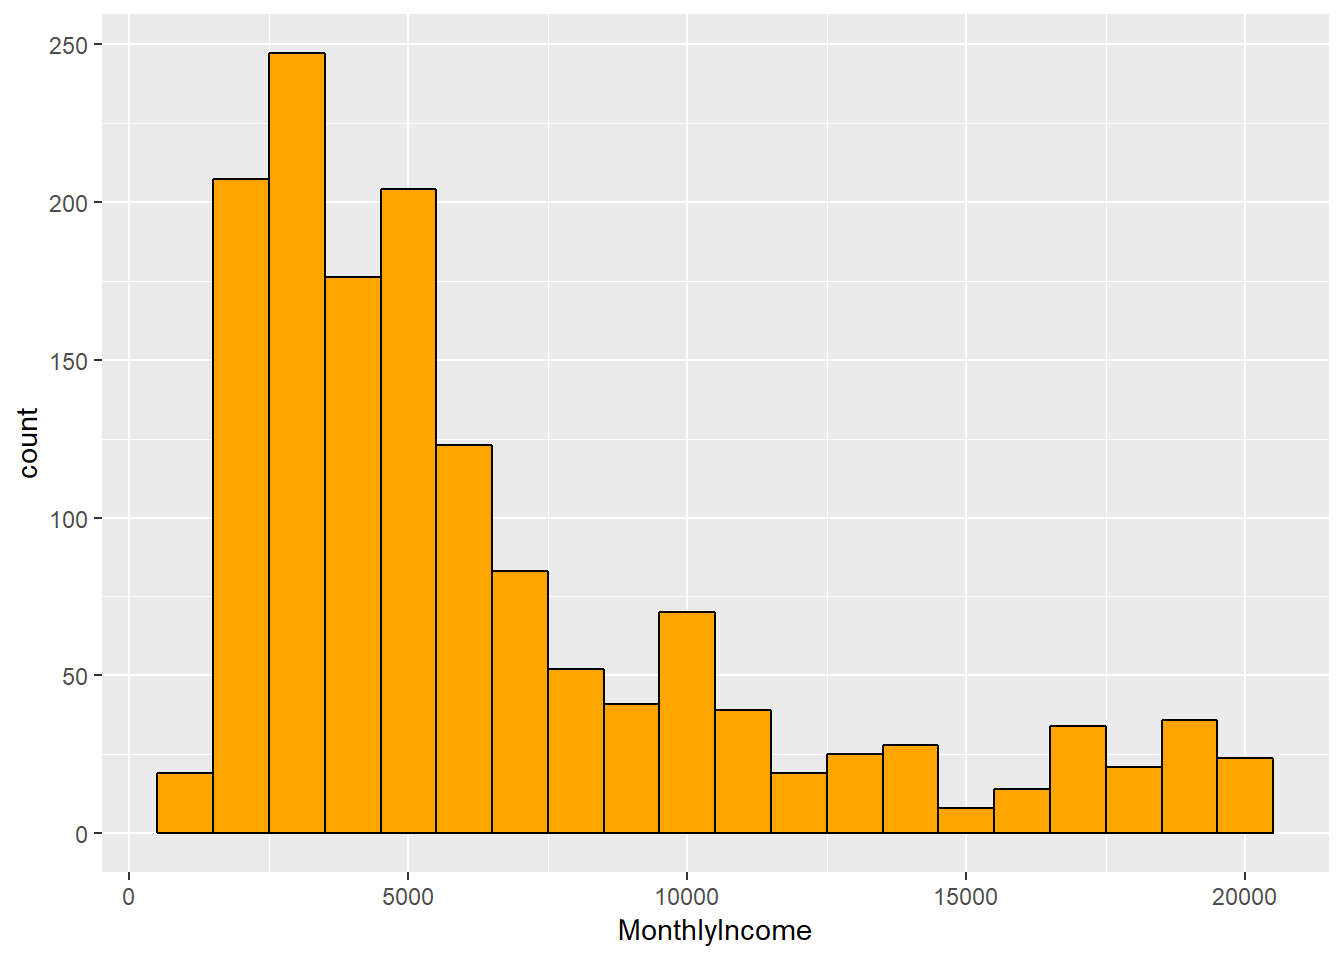
\includegraphics{DDSAnalytics_Case_Study_files/figure-latex/uni_non_cat_demo_work-1.pdf}

\subsubsection{Observations}\label{observations-2}

\begin{itemize}
\tightlist
\item
  All data for these observations is right skewed. Transformation of
  data may be needed for further analysis
\end{itemize}

\subsection{Univariate EDA - Categorical
Variables}\label{univariate-eda---categorical-variables}

\subsubsection{Employee Demographics -
Personal}\label{employee-demographics---personal}

\begin{Shaded}
\begin{Highlighting}[]
\CommentTok{#Investigate personal demographics in the data such as gender, education marital status, etc. }
\CommentTok{#Gender}
\NormalTok{p1 =}\StringTok{ }\NormalTok{empDF }\OperatorTok
\StringTok{  }\KeywordTok{group_by}\NormalTok{(Gender) }\OperatorTok
\StringTok{  }\NormalTok{dplyr}\OperatorTok{::}\KeywordTok{summarise}\NormalTok{(}\DataTypeTok{counts =} \KeywordTok{n}\NormalTok{()) }\OperatorTok
\StringTok{  }\KeywordTok{ggplot}\NormalTok{(}\KeywordTok{aes}\NormalTok{(}\DataTypeTok{x =} \KeywordTok{as.factor}\NormalTok{(Gender), }\DataTypeTok{y =}\NormalTok{ counts)) }\OperatorTok{+}\StringTok{ }\KeywordTok{geom_bar}\NormalTok{(}\DataTypeTok{stat =} \StringTok{'identity'}\NormalTok{, }\DataTypeTok{fill =} \StringTok{"coral1"}\NormalTok{) }\OperatorTok{+}\StringTok{ }\KeywordTok{ggtitle}\NormalTok{(}\StringTok{"Gender"}\NormalTok{) }\OperatorTok{+}\KeywordTok{geom_text}\NormalTok{(}\KeywordTok{aes}\NormalTok{(}\DataTypeTok{label=}\NormalTok{counts), }\DataTypeTok{size =} \FloatTok{2.5}\NormalTok{, }\DataTypeTok{position=}\KeywordTok{position_dodge}\NormalTok{(}\DataTypeTok{width=}\FloatTok{0.2}\NormalTok{), }\DataTypeTok{vjust=}\OperatorTok{-}\FloatTok{0.25}\NormalTok{) }\OperatorTok{+}\StringTok{ }\KeywordTok{theme}\NormalTok{(}\DataTypeTok{plot.title =} \KeywordTok{element_text}\NormalTok{(}\DataTypeTok{size =}\DecValTok{10}\NormalTok{),}\DataTypeTok{axis.text.x =} \KeywordTok{element_text}\NormalTok{(}\DataTypeTok{size =}\DecValTok{7}\NormalTok{,}\DataTypeTok{angle =} \DecValTok{45}\NormalTok{, }\DataTypeTok{hjust =} \DecValTok{1}\NormalTok{),}\DataTypeTok{axis.title.x=}\KeywordTok{element_blank}\NormalTok{()) }\OperatorTok{+}\StringTok{ }\KeywordTok{scale_y_continuous}\NormalTok{(}\DataTypeTok{limits =} \KeywordTok{c}\NormalTok{(}\DecValTok{0}\NormalTok{, }\DecValTok{900}\NormalTok{))}

\CommentTok{#Education}
\NormalTok{p2 =}\StringTok{ }\NormalTok{empDF }\OperatorTok
\StringTok{  }\KeywordTok{group_by}\NormalTok{(Education) }\OperatorTok
\StringTok{  }\NormalTok{dplyr}\OperatorTok{::}\KeywordTok{summarise}\NormalTok{(}\DataTypeTok{counts =} \KeywordTok{n}\NormalTok{()) }\OperatorTok
\StringTok{  }\KeywordTok{ggplot}\NormalTok{(}\KeywordTok{aes}\NormalTok{(}\DataTypeTok{x =} \KeywordTok{as.factor}\NormalTok{(Education), }\DataTypeTok{y =}\NormalTok{ counts)) }\OperatorTok{+}\StringTok{ }\KeywordTok{geom_bar}\NormalTok{(}\DataTypeTok{stat =} \StringTok{'identity'}\NormalTok{, }\DataTypeTok{fill =} \StringTok{"coral1"}\NormalTok{) }\OperatorTok{+}\StringTok{ }\KeywordTok{ggtitle}\NormalTok{(}\StringTok{"Education"}\NormalTok{) }\OperatorTok{+}\KeywordTok{geom_text}\NormalTok{(}\KeywordTok{aes}\NormalTok{(}\DataTypeTok{label=}\NormalTok{counts), }\DataTypeTok{size =} \FloatTok{2.5}\NormalTok{, }\DataTypeTok{position=}\KeywordTok{position_dodge}\NormalTok{(}\DataTypeTok{width=}\FloatTok{0.2}\NormalTok{), }\DataTypeTok{vjust=}\OperatorTok{-}\FloatTok{0.25}\NormalTok{) }\OperatorTok{+}\StringTok{ }\KeywordTok{theme}\NormalTok{(}\DataTypeTok{plot.title =} \KeywordTok{element_text}\NormalTok{(}\DataTypeTok{size =}\DecValTok{10}\NormalTok{),}\DataTypeTok{axis.text.x =} \KeywordTok{element_text}\NormalTok{(}\DataTypeTok{size =}\DecValTok{7}\NormalTok{,}\DataTypeTok{angle =} \DecValTok{45}\NormalTok{, }\DataTypeTok{hjust =} \DecValTok{1}\NormalTok{),}\DataTypeTok{axis.title.x=}\KeywordTok{element_blank}\NormalTok{()) }\OperatorTok{+}\StringTok{ }\KeywordTok{scale_y_continuous}\NormalTok{(}\DataTypeTok{limits =} \KeywordTok{c}\NormalTok{(}\DecValTok{0}\NormalTok{, }\DecValTok{650}\NormalTok{))}

\CommentTok{#Education Field}
\NormalTok{p3 =}\StringTok{ }\NormalTok{empDF }\OperatorTok
\StringTok{  }\KeywordTok{group_by}\NormalTok{(EducationField) }\OperatorTok
\StringTok{ }\NormalTok{dplyr}\OperatorTok{::}\KeywordTok{summarise}\NormalTok{(}\DataTypeTok{counts =} \KeywordTok{n}\NormalTok{()) }\OperatorTok
\StringTok{  }\KeywordTok{ggplot}\NormalTok{(}\KeywordTok{aes}\NormalTok{(}\DataTypeTok{x =} \KeywordTok{as.factor}\NormalTok{(EducationField), }\DataTypeTok{y =}\NormalTok{ counts)) }\OperatorTok{+}\StringTok{ }\KeywordTok{geom_bar}\NormalTok{(}\DataTypeTok{stat =} \StringTok{'identity'}\NormalTok{, }\DataTypeTok{fill =} \StringTok{"coral1"}\NormalTok{) }\OperatorTok{+}\StringTok{ }\KeywordTok{ggtitle}\NormalTok{(}\StringTok{"Education Field"}\NormalTok{) }\OperatorTok{+}\KeywordTok{geom_text}\NormalTok{(}\KeywordTok{aes}\NormalTok{(}\DataTypeTok{label=}\NormalTok{counts), }\DataTypeTok{size =} \FloatTok{2.5}\NormalTok{, }\DataTypeTok{position=}\KeywordTok{position_dodge}\NormalTok{(}\DataTypeTok{width=}\FloatTok{0.2}\NormalTok{), }\DataTypeTok{vjust=}\OperatorTok{-}\FloatTok{0.25}\NormalTok{) }\OperatorTok{+}\StringTok{ }\KeywordTok{theme}\NormalTok{(}\DataTypeTok{plot.title =} \KeywordTok{element_text}\NormalTok{(}\DataTypeTok{size =}\DecValTok{10}\NormalTok{),}\DataTypeTok{axis.text.x =} \KeywordTok{element_text}\NormalTok{(}\DataTypeTok{size =}\DecValTok{7}\NormalTok{,}\DataTypeTok{angle =} \DecValTok{45}\NormalTok{, }\DataTypeTok{hjust =} \DecValTok{1}\NormalTok{),}\DataTypeTok{axis.title.x=}\KeywordTok{element_blank}\NormalTok{()) }\OperatorTok{+}\StringTok{ }\KeywordTok{scale_y_continuous}\NormalTok{(}\DataTypeTok{limits =} \KeywordTok{c}\NormalTok{(}\DecValTok{0}\NormalTok{, }\DecValTok{650}\NormalTok{))}

\CommentTok{#Marital Status}
\NormalTok{p4 =}\StringTok{ }\NormalTok{empDF }\OperatorTok
\StringTok{  }\KeywordTok{group_by}\NormalTok{(MaritalStatus) }\OperatorTok
\StringTok{  }\NormalTok{dplyr}\OperatorTok{::}\KeywordTok{summarise}\NormalTok{(}\DataTypeTok{counts =} \KeywordTok{n}\NormalTok{()) }\OperatorTok
\StringTok{  }\KeywordTok{ggplot}\NormalTok{(}\KeywordTok{aes}\NormalTok{(}\DataTypeTok{x =} \KeywordTok{as.factor}\NormalTok{(MaritalStatus), }\DataTypeTok{y =}\NormalTok{ counts)) }\OperatorTok{+}\StringTok{ }\KeywordTok{geom_bar}\NormalTok{(}\DataTypeTok{stat =} \StringTok{'identity'}\NormalTok{, }\DataTypeTok{fill =} \StringTok{"coral1"}\NormalTok{)}\OperatorTok{+}\StringTok{ }\KeywordTok{ggtitle}\NormalTok{(}\StringTok{"Marital Status"}\NormalTok{) }\OperatorTok{+}\KeywordTok{geom_text}\NormalTok{(}\KeywordTok{aes}\NormalTok{(}\DataTypeTok{label=}\NormalTok{counts), }\DataTypeTok{size =} \FloatTok{2.5}\NormalTok{, }\DataTypeTok{position=}\KeywordTok{position_dodge}\NormalTok{(}\DataTypeTok{width=}\FloatTok{0.2}\NormalTok{), }\DataTypeTok{vjust=}\OperatorTok{-}\FloatTok{0.25}\NormalTok{) }\OperatorTok{+}\StringTok{ }\KeywordTok{theme}\NormalTok{(}\DataTypeTok{plot.title =} \KeywordTok{element_text}\NormalTok{(}\DataTypeTok{size =}\DecValTok{10}\NormalTok{),}\DataTypeTok{axis.text.x =} \KeywordTok{element_text}\NormalTok{(}\DataTypeTok{size =}\DecValTok{7}\NormalTok{,}\DataTypeTok{angle =} \DecValTok{45}\NormalTok{, }\DataTypeTok{hjust =} \DecValTok{1}\NormalTok{),}\DataTypeTok{axis.title.x=}\KeywordTok{element_blank}\NormalTok{()) }\OperatorTok{+}\StringTok{ }\KeywordTok{scale_y_continuous}\NormalTok{(}\DataTypeTok{limits =} \KeywordTok{c}\NormalTok{(}\DecValTok{0}\NormalTok{, }\DecValTok{750}\NormalTok{))}

\CommentTok{#Relationship Satisfaction}
\NormalTok{p5 =}\StringTok{ }\NormalTok{empDF }\OperatorTok
\StringTok{  }\KeywordTok{group_by}\NormalTok{(RelationshipSatisfaction) }\OperatorTok
\StringTok{  }\NormalTok{dplyr}\OperatorTok{::}\KeywordTok{summarise}\NormalTok{(}\DataTypeTok{counts =} \KeywordTok{n}\NormalTok{()) }\OperatorTok
\StringTok{  }\KeywordTok{ggplot}\NormalTok{(}\KeywordTok{aes}\NormalTok{(}\DataTypeTok{x =} \KeywordTok{as.factor}\NormalTok{(RelationshipSatisfaction), }\DataTypeTok{y =}\NormalTok{ counts)) }\OperatorTok{+}\StringTok{ }\KeywordTok{geom_bar}\NormalTok{(}\DataTypeTok{stat =} \StringTok{'identity'}\NormalTok{, }\DataTypeTok{fill =} \StringTok{"coral1"}\NormalTok{) }\OperatorTok{+}\StringTok{ }\KeywordTok{ggtitle}\NormalTok{(}\StringTok{"Relationship Satisfaction"}\NormalTok{) }\OperatorTok{+}\KeywordTok{geom_text}\NormalTok{(}\KeywordTok{aes}\NormalTok{(}\DataTypeTok{label=}\NormalTok{counts), }\DataTypeTok{size =} \FloatTok{2.5}\NormalTok{, }\DataTypeTok{position=}\KeywordTok{position_dodge}\NormalTok{(}\DataTypeTok{width=}\FloatTok{0.2}\NormalTok{), }\DataTypeTok{vjust=}\OperatorTok{-}\FloatTok{0.25}\NormalTok{) }\OperatorTok{+}\StringTok{ }\KeywordTok{theme}\NormalTok{(}\DataTypeTok{plot.title =} \KeywordTok{element_text}\NormalTok{(}\DataTypeTok{size =}\DecValTok{10}\NormalTok{),}\DataTypeTok{axis.text.x =} \KeywordTok{element_text}\NormalTok{(}\DataTypeTok{size =}\DecValTok{7}\NormalTok{,}\DataTypeTok{angle =} \DecValTok{45}\NormalTok{, }\DataTypeTok{hjust =} \DecValTok{1}\NormalTok{),}\DataTypeTok{axis.title.x=}\KeywordTok{element_blank}\NormalTok{())}\OperatorTok{+}\StringTok{ }\KeywordTok{scale_y_continuous}\NormalTok{(}\DataTypeTok{limits =} \KeywordTok{c}\NormalTok{(}\DecValTok{0}\NormalTok{, }\DecValTok{500}\NormalTok{))}

\CommentTok{#Work Life Balance}
\NormalTok{p6 =}\StringTok{ }\NormalTok{empDF }\OperatorTok
\StringTok{  }\KeywordTok{group_by}\NormalTok{(WorkLifeBalance) }\OperatorTok
\StringTok{  }\NormalTok{dplyr}\OperatorTok{::}\KeywordTok{summarise}\NormalTok{(}\DataTypeTok{counts =} \KeywordTok{n}\NormalTok{()) }\OperatorTok
\StringTok{  }\KeywordTok{ggplot}\NormalTok{(}\KeywordTok{aes}\NormalTok{(}\DataTypeTok{x =} \KeywordTok{as.factor}\NormalTok{(WorkLifeBalance), }\DataTypeTok{y =}\NormalTok{ counts)) }\OperatorTok{+}\StringTok{ }\KeywordTok{geom_bar}\NormalTok{(}\DataTypeTok{stat =} \StringTok{'identity'}\NormalTok{, }\DataTypeTok{fill =} \StringTok{"coral1"}\NormalTok{)}\OperatorTok{+}\StringTok{ }\KeywordTok{ggtitle}\NormalTok{(}\StringTok{"Work Life Balance"}\NormalTok{) }\OperatorTok{+}\KeywordTok{geom_text}\NormalTok{(}\KeywordTok{aes}\NormalTok{(}\DataTypeTok{label=}\NormalTok{counts), }\DataTypeTok{size =} \FloatTok{2.5}\NormalTok{, }\DataTypeTok{position=}\KeywordTok{position_dodge}\NormalTok{(}\DataTypeTok{width=}\FloatTok{0.2}\NormalTok{), }\DataTypeTok{vjust=}\OperatorTok{-}\FloatTok{0.25}\NormalTok{) }\OperatorTok{+}\StringTok{ }\KeywordTok{theme}\NormalTok{(}\DataTypeTok{plot.title =} \KeywordTok{element_text}\NormalTok{(}\DataTypeTok{size =}\DecValTok{10}\NormalTok{),}\DataTypeTok{axis.text.x =} \KeywordTok{element_text}\NormalTok{(}\DataTypeTok{size =}\DecValTok{7}\NormalTok{,}\DataTypeTok{angle =} \DecValTok{45}\NormalTok{, }\DataTypeTok{hjust =} \DecValTok{1}\NormalTok{),}\DataTypeTok{axis.title.x=}\KeywordTok{element_blank}\NormalTok{()) }\OperatorTok{+}\StringTok{ }\KeywordTok{scale_y_continuous}\NormalTok{(}\DataTypeTok{limits =} \KeywordTok{c}\NormalTok{(}\DecValTok{0}\NormalTok{, }\DecValTok{950}\NormalTok{))}

\KeywordTok{ggarrange}\NormalTok{(p1,p2,p3,p4,p5,p6)}
\end{Highlighting}
\end{Shaded}

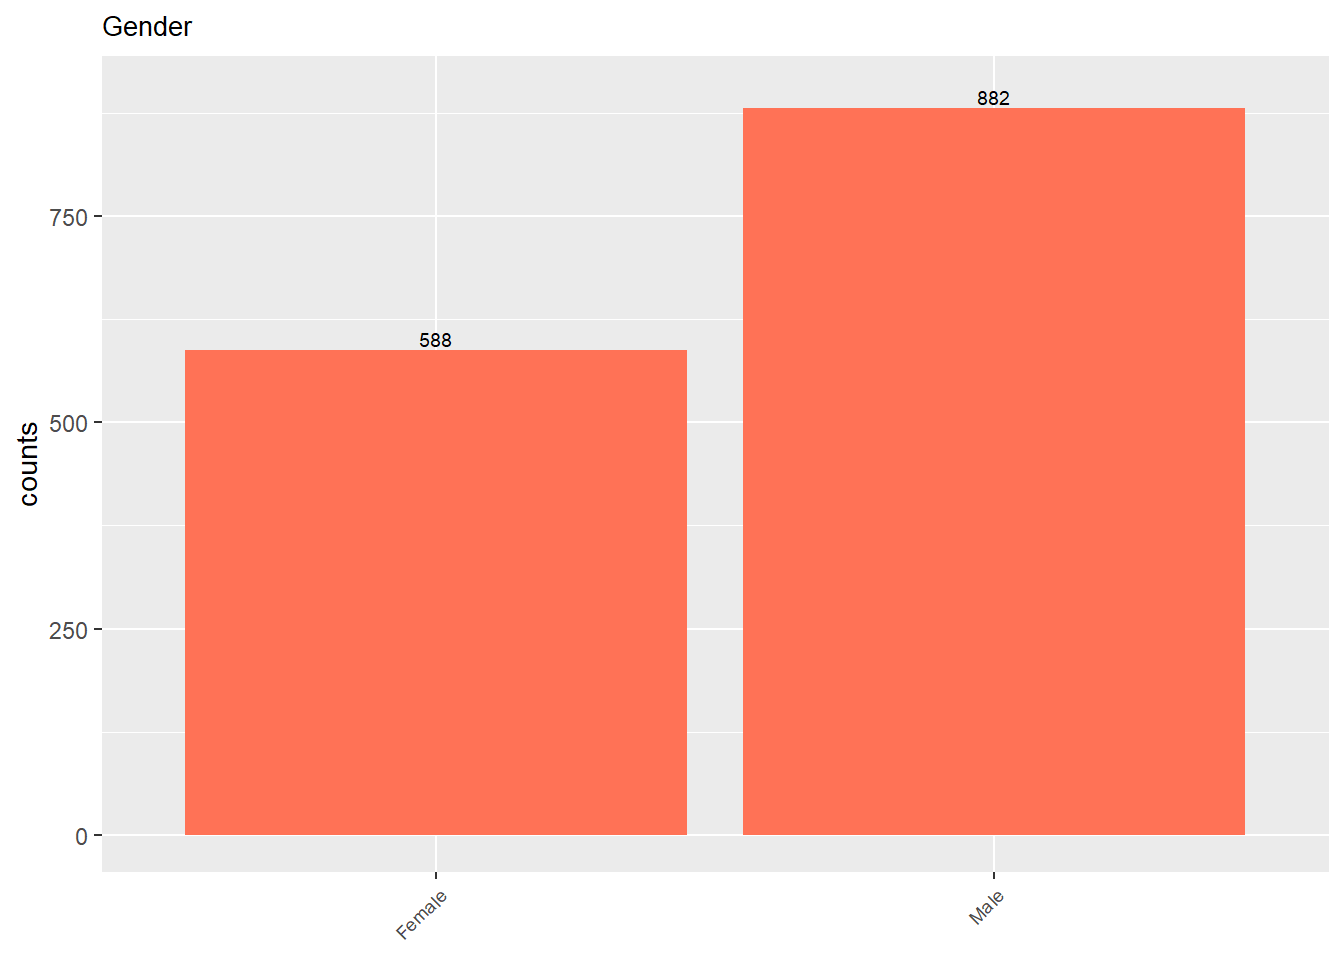
\includegraphics{DDSAnalytics_Case_Study_files/figure-latex/uni_cat_demo_personal-1.pdf}

\subsubsection{Observations:}\label{observations-3}

\begin{itemize}
\tightlist
\item
  Approximately 60\% of the employees are male.
\item
  Approximately 39\% of the employees have a bachelors degree, with 27\%
  having a masters degree.
\item
  Approximately 41\% of the employees have a life sciences degree.
\item
  Approximately 76\% of the employees have a life science or medical
  degree.
\item
  Approximately 46\% of the employees are married, with 32\% being
  single.
\item
  More than 30\% of the employees rate Relationship Satisfaction as High
  or Very High.
\item
  More than 60\% of the employees rate Work Life Balance as Better.
\end{itemize}

\subsubsection{Employee Demographics - Work
Environment}\label{employee-demographics---work-environment-1}

\begin{Shaded}
\begin{Highlighting}[]
\CommentTok{#Investigate work environment categorical variables such as Business Travel, Overtime, etc}

\CommentTok{#Business Travel}
\NormalTok{p1 =}\StringTok{ }\NormalTok{empDF }\OperatorTok
\StringTok{  }\KeywordTok{group_by}\NormalTok{(BusinessTravel) }\OperatorTok
\StringTok{  }\NormalTok{dplyr}\OperatorTok{::}\KeywordTok{summarise}\NormalTok{(}\DataTypeTok{counts =} \KeywordTok{n}\NormalTok{()) }\OperatorTok
\StringTok{  }\KeywordTok{ggplot}\NormalTok{(}\KeywordTok{aes}\NormalTok{(}\DataTypeTok{x =} \KeywordTok{as.factor}\NormalTok{(BusinessTravel), }\DataTypeTok{y =}\NormalTok{ counts)) }\OperatorTok{+}\StringTok{ }\KeywordTok{geom_bar}\NormalTok{(}\DataTypeTok{stat =} \StringTok{'identity'}\NormalTok{, }\DataTypeTok{fill =} \StringTok{"coral1"}\NormalTok{) }\OperatorTok{+}\StringTok{ }\KeywordTok{ggtitle}\NormalTok{(}\StringTok{"Business Travel"}\NormalTok{) }\OperatorTok{+}\KeywordTok{geom_text}\NormalTok{(}\KeywordTok{aes}\NormalTok{(}\DataTypeTok{label=}\NormalTok{counts), }\DataTypeTok{size =} \FloatTok{2.5}\NormalTok{, }\DataTypeTok{position=}\KeywordTok{position_dodge}\NormalTok{(}\DataTypeTok{width=}\FloatTok{0.2}\NormalTok{), }\DataTypeTok{vjust=}\OperatorTok{-}\FloatTok{0.25}\NormalTok{)}\OperatorTok{+}\StringTok{ }\KeywordTok{theme}\NormalTok{(}\DataTypeTok{plot.title =} \KeywordTok{element_text}\NormalTok{(}\DataTypeTok{size =}\DecValTok{10}\NormalTok{),}\DataTypeTok{axis.text.x =} \KeywordTok{element_text}\NormalTok{(}\DataTypeTok{size =}\DecValTok{10}\NormalTok{,}\DataTypeTok{angle =} \DecValTok{45}\NormalTok{, }\DataTypeTok{hjust =} \DecValTok{1}\NormalTok{),}\DataTypeTok{axis.title.x=}\KeywordTok{element_blank}\NormalTok{())}\OperatorTok{+}\StringTok{ }\KeywordTok{scale_y_continuous}\NormalTok{(}\DataTypeTok{limits =} \KeywordTok{c}\NormalTok{(}\DecValTok{0}\NormalTok{, }\DecValTok{1100}\NormalTok{))}

\CommentTok{#Environmental Satisfaction}
\NormalTok{p2 =}\StringTok{ }\NormalTok{empDF }\OperatorTok
\StringTok{  }\KeywordTok{group_by}\NormalTok{(EnvironmentSatisfaction) }\OperatorTok
\StringTok{  }\NormalTok{dplyr}\OperatorTok{::}\KeywordTok{summarise}\NormalTok{(}\DataTypeTok{counts =} \KeywordTok{n}\NormalTok{()) }\OperatorTok
\StringTok{  }\KeywordTok{ggplot}\NormalTok{(}\KeywordTok{aes}\NormalTok{(}\DataTypeTok{x =} \KeywordTok{as.factor}\NormalTok{(EnvironmentSatisfaction), }\DataTypeTok{y =}\NormalTok{ counts)) }\OperatorTok{+}\StringTok{ }\KeywordTok{geom_bar}\NormalTok{(}\DataTypeTok{stat =} \StringTok{'identity'}\NormalTok{, }\DataTypeTok{fill =} \StringTok{"coral1"}\NormalTok{) }\OperatorTok{+}\StringTok{ }\KeywordTok{ggtitle}\NormalTok{(}\StringTok{"Environment Satisfaction"}\NormalTok{) }\OperatorTok{+}\StringTok{ }\KeywordTok{geom_text}\NormalTok{(}\KeywordTok{aes}\NormalTok{(}\DataTypeTok{label=}\NormalTok{counts), }\DataTypeTok{size =} \FloatTok{2.5}\NormalTok{, }\DataTypeTok{position=}\KeywordTok{position_dodge}\NormalTok{(}\DataTypeTok{width=}\FloatTok{0.2}\NormalTok{), }\DataTypeTok{vjust=}\OperatorTok{-}\FloatTok{0.25}\NormalTok{) }\OperatorTok{+}\StringTok{ }\KeywordTok{theme}\NormalTok{(}\DataTypeTok{plot.title =} \KeywordTok{element_text}\NormalTok{(}\DataTypeTok{size =}\DecValTok{10}\NormalTok{),}\DataTypeTok{axis.text.x =} \KeywordTok{element_text}\NormalTok{(}\DataTypeTok{size =}\DecValTok{10}\NormalTok{,}\DataTypeTok{angle =} \DecValTok{45}\NormalTok{, }\DataTypeTok{hjust =} \DecValTok{1}\NormalTok{),}\DataTypeTok{axis.title.x=}\KeywordTok{element_blank}\NormalTok{()) }\OperatorTok{+}\StringTok{ }\KeywordTok{scale_y_continuous}\NormalTok{(}\DataTypeTok{limits =} \KeywordTok{c}\NormalTok{(}\DecValTok{0}\NormalTok{, }\DecValTok{500}\NormalTok{))}

\CommentTok{#Job Involvement}
\NormalTok{p3 =}\StringTok{ }\NormalTok{empDF }\OperatorTok
\StringTok{  }\KeywordTok{group_by}\NormalTok{(JobInvolvement) }\OperatorTok
\StringTok{ }\NormalTok{dplyr}\OperatorTok{::}\KeywordTok{summarise}\NormalTok{(}\DataTypeTok{counts =} \KeywordTok{n}\NormalTok{()) }\OperatorTok
\StringTok{  }\KeywordTok{ggplot}\NormalTok{(}\KeywordTok{aes}\NormalTok{(}\DataTypeTok{x =} \KeywordTok{as.factor}\NormalTok{(JobInvolvement), }\DataTypeTok{y =}\NormalTok{ counts)) }\OperatorTok{+}\StringTok{ }\KeywordTok{geom_bar}\NormalTok{(}\DataTypeTok{stat =} \StringTok{'identity'}\NormalTok{, }\DataTypeTok{fill =} \StringTok{"coral1"}\NormalTok{) }\OperatorTok{+}\StringTok{ }\KeywordTok{ggtitle}\NormalTok{(}\StringTok{"Job Involvement"}\NormalTok{) }\OperatorTok{+}\KeywordTok{geom_text}\NormalTok{(}\KeywordTok{aes}\NormalTok{(}\DataTypeTok{label=}\NormalTok{counts), }\DataTypeTok{size =} \FloatTok{2.5}\NormalTok{, }\DataTypeTok{position=}\KeywordTok{position_dodge}\NormalTok{(}\DataTypeTok{width=}\FloatTok{0.2}\NormalTok{), }\DataTypeTok{vjust=}\OperatorTok{-}\FloatTok{0.25}\NormalTok{)}\OperatorTok{+}\StringTok{ }\KeywordTok{theme}\NormalTok{(}\DataTypeTok{plot.title =} \KeywordTok{element_text}\NormalTok{(}\DataTypeTok{size =}\DecValTok{10}\NormalTok{),}\DataTypeTok{axis.text.x =} \KeywordTok{element_text}\NormalTok{(}\DataTypeTok{size =}\DecValTok{10}\NormalTok{,}\DataTypeTok{angle =} \DecValTok{45}\NormalTok{, }\DataTypeTok{hjust =} \DecValTok{1}\NormalTok{),}\DataTypeTok{axis.title.x=}\KeywordTok{element_blank}\NormalTok{()) }\OperatorTok{+}\StringTok{ }\KeywordTok{scale_y_continuous}\NormalTok{(}\DataTypeTok{limits =} \KeywordTok{c}\NormalTok{(}\DecValTok{0}\NormalTok{, }\DecValTok{900}\NormalTok{))}

\CommentTok{#Job Satisfaction}
\NormalTok{p4 =}\StringTok{ }\NormalTok{empDF }\OperatorTok
\StringTok{  }\KeywordTok{group_by}\NormalTok{(JobSatisfaction) }\OperatorTok
\StringTok{  }\NormalTok{dplyr}\OperatorTok{::}\KeywordTok{summarise}\NormalTok{(}\DataTypeTok{counts =} \KeywordTok{n}\NormalTok{()) }\OperatorTok
\StringTok{  }\KeywordTok{ggplot}\NormalTok{(}\KeywordTok{aes}\NormalTok{(}\DataTypeTok{x =} \KeywordTok{as.factor}\NormalTok{(JobSatisfaction), }\DataTypeTok{y =}\NormalTok{ counts)) }\OperatorTok{+}\StringTok{ }\KeywordTok{geom_bar}\NormalTok{(}\DataTypeTok{stat =} \StringTok{'identity'}\NormalTok{, }\DataTypeTok{fill =} \StringTok{"coral1"}\NormalTok{) }\OperatorTok{+}\StringTok{ }\KeywordTok{ggtitle}\NormalTok{(}\StringTok{"Job Satisfaction"}\NormalTok{) }\OperatorTok{+}\KeywordTok{geom_text}\NormalTok{(}\KeywordTok{aes}\NormalTok{(}\DataTypeTok{label=}\NormalTok{counts), }\DataTypeTok{size =} \FloatTok{2.5}\NormalTok{, }\DataTypeTok{position=}\KeywordTok{position_dodge}\NormalTok{(}\DataTypeTok{width=}\FloatTok{0.2}\NormalTok{), }\DataTypeTok{vjust=}\OperatorTok{-}\FloatTok{0.25}\NormalTok{) }\OperatorTok{+}\StringTok{ }\KeywordTok{theme}\NormalTok{(}\DataTypeTok{plot.title =} \KeywordTok{element_text}\NormalTok{(}\DataTypeTok{size =}\DecValTok{10}\NormalTok{),}\DataTypeTok{axis.text.x =} \KeywordTok{element_text}\NormalTok{(}\DataTypeTok{size =}\DecValTok{7}\NormalTok{,}\DataTypeTok{angle =} \DecValTok{45}\NormalTok{, }\DataTypeTok{hjust =} \DecValTok{1}\NormalTok{),}\DataTypeTok{axis.title.x=}\KeywordTok{element_blank}\NormalTok{()) }\OperatorTok{+}\StringTok{ }\KeywordTok{scale_y_continuous}\NormalTok{(}\DataTypeTok{limits =} \KeywordTok{c}\NormalTok{(}\DecValTok{0}\NormalTok{, }\DecValTok{500}\NormalTok{))}

\CommentTok{#Over Time}
\NormalTok{p5 =}\StringTok{ }\NormalTok{empDF }\OperatorTok
\StringTok{  }\KeywordTok{group_by}\NormalTok{(OverTime) }\OperatorTok
\StringTok{  }\NormalTok{dplyr}\OperatorTok{::}\KeywordTok{summarise}\NormalTok{(}\DataTypeTok{counts =} \KeywordTok{n}\NormalTok{()) }\OperatorTok
\StringTok{  }\KeywordTok{ggplot}\NormalTok{(}\KeywordTok{aes}\NormalTok{(}\DataTypeTok{x =} \KeywordTok{as.factor}\NormalTok{(OverTime), }\DataTypeTok{y =}\NormalTok{ counts)) }\OperatorTok{+}\StringTok{ }\KeywordTok{geom_bar}\NormalTok{(}\DataTypeTok{stat =} \StringTok{'identity'}\NormalTok{, }\DataTypeTok{fill =} \StringTok{"coral1"}\NormalTok{) }\OperatorTok{+}\StringTok{ }\KeywordTok{ggtitle}\NormalTok{(}\StringTok{"Over Time"}\NormalTok{) }\OperatorTok{+}\KeywordTok{geom_text}\NormalTok{(}\KeywordTok{aes}\NormalTok{(}\DataTypeTok{label=}\NormalTok{counts), }\DataTypeTok{size =} \FloatTok{2.5}\NormalTok{, }\DataTypeTok{position=}\KeywordTok{position_dodge}\NormalTok{(}\DataTypeTok{width=}\FloatTok{0.2}\NormalTok{), }\DataTypeTok{vjust=}\OperatorTok{-}\FloatTok{0.25}\NormalTok{)}\OperatorTok{+}\StringTok{ }\KeywordTok{theme}\NormalTok{(}\DataTypeTok{plot.title =} \KeywordTok{element_text}\NormalTok{(}\DataTypeTok{size =}\DecValTok{10}\NormalTok{),}\DataTypeTok{axis.text.x =} \KeywordTok{element_text}\NormalTok{(}\DataTypeTok{size =}\DecValTok{7}\NormalTok{,}\DataTypeTok{angle =} \DecValTok{45}\NormalTok{, }\DataTypeTok{hjust =} \DecValTok{1}\NormalTok{),}\DataTypeTok{axis.title.x=}\KeywordTok{element_blank}\NormalTok{()) }\OperatorTok{+}\StringTok{ }\KeywordTok{scale_y_continuous}\NormalTok{(}\DataTypeTok{limits =} \KeywordTok{c}\NormalTok{(}\DecValTok{0}\NormalTok{, }\DecValTok{1100}\NormalTok{))}

\CommentTok{#Performance Rating}
\NormalTok{p6 =}\StringTok{ }\NormalTok{empDF }\OperatorTok
\StringTok{  }\KeywordTok{group_by}\NormalTok{(PerformanceRating) }\OperatorTok
\StringTok{  }\NormalTok{dplyr}\OperatorTok{::}\KeywordTok{summarise}\NormalTok{(}\DataTypeTok{counts =} \KeywordTok{n}\NormalTok{()) }\OperatorTok
\StringTok{  }\KeywordTok{ggplot}\NormalTok{(}\KeywordTok{aes}\NormalTok{(}\DataTypeTok{x =} \KeywordTok{as.factor}\NormalTok{(PerformanceRating), }\DataTypeTok{y =}\NormalTok{ counts)) }\OperatorTok{+}\StringTok{ }\KeywordTok{geom_bar}\NormalTok{(}\DataTypeTok{stat =} \StringTok{'identity'}\NormalTok{, }\DataTypeTok{fill =} \StringTok{"coral1"}\NormalTok{) }\OperatorTok{+}\StringTok{ }\KeywordTok{ggtitle}\NormalTok{(}\StringTok{"Performance Rating"}\NormalTok{) }\OperatorTok{+}\KeywordTok{geom_text}\NormalTok{(}\KeywordTok{aes}\NormalTok{(}\DataTypeTok{label=}\NormalTok{counts), }\DataTypeTok{size =} \FloatTok{2.5}\NormalTok{, }\DataTypeTok{position=}\KeywordTok{position_dodge}\NormalTok{(}\DataTypeTok{width=}\FloatTok{0.2}\NormalTok{), }\DataTypeTok{vjust=}\OperatorTok{-}\FloatTok{0.25}\NormalTok{)}\OperatorTok{+}\StringTok{ }\KeywordTok{theme}\NormalTok{(}\DataTypeTok{plot.title =} \KeywordTok{element_text}\NormalTok{(}\DataTypeTok{size =}\DecValTok{10}\NormalTok{),}\DataTypeTok{axis.text.x =} \KeywordTok{element_text}\NormalTok{(}\DataTypeTok{size =}\DecValTok{7}\NormalTok{,}\DataTypeTok{angle =} \DecValTok{45}\NormalTok{, }\DataTypeTok{hjust =} \DecValTok{1}\NormalTok{),}\DataTypeTok{axis.title.x=}\KeywordTok{element_blank}\NormalTok{()) }\OperatorTok{+}\StringTok{ }\KeywordTok{scale_y_continuous}\NormalTok{(}\DataTypeTok{limits =} \KeywordTok{c}\NormalTok{(}\DecValTok{0}\NormalTok{, }\DecValTok{1300}\NormalTok{))}

\CommentTok{#Employee By Department}
\NormalTok{p7 =}\StringTok{ }\NormalTok{empDF }\OperatorTok
\StringTok{  }\KeywordTok{group_by}\NormalTok{(Department) }\OperatorTok
\StringTok{  }\NormalTok{dplyr}\OperatorTok{::}\KeywordTok{summarise}\NormalTok{(}\DataTypeTok{counts =} \KeywordTok{n}\NormalTok{()) }\OperatorTok
\StringTok{  }\KeywordTok{ggplot}\NormalTok{(}\KeywordTok{aes}\NormalTok{(}\DataTypeTok{x =} \KeywordTok{as.factor}\NormalTok{(Department), }\DataTypeTok{y =}\NormalTok{ counts)) }\OperatorTok{+}\StringTok{ }\KeywordTok{geom_bar}\NormalTok{(}\DataTypeTok{stat =} \StringTok{'identity'}\NormalTok{, }\DataTypeTok{fill =} \StringTok{"coral1"}\NormalTok{) }\OperatorTok{+}\StringTok{ }\KeywordTok{ggtitle}\NormalTok{(}\StringTok{"Department"}\NormalTok{) }\OperatorTok{+}\KeywordTok{geom_text}\NormalTok{(}\KeywordTok{aes}\NormalTok{(}\DataTypeTok{label=}\NormalTok{counts), }\DataTypeTok{size =} \FloatTok{2.5}\NormalTok{, }\DataTypeTok{position=}\KeywordTok{position_dodge}\NormalTok{(}\DataTypeTok{width=}\FloatTok{0.2}\NormalTok{), }\DataTypeTok{vjust=}\OperatorTok{-}\FloatTok{0.25}\NormalTok{)}\OperatorTok{+}\StringTok{ }\KeywordTok{theme}\NormalTok{(}\DataTypeTok{plot.title =} \KeywordTok{element_text}\NormalTok{(}\DataTypeTok{size =}\DecValTok{10}\NormalTok{),}\DataTypeTok{axis.text.x =} \KeywordTok{element_text}\NormalTok{(}\DataTypeTok{size =} \DecValTok{7}\NormalTok{, }\DataTypeTok{angle =} \DecValTok{45}\NormalTok{, }\DataTypeTok{hjust =} \DecValTok{1}\NormalTok{),}\DataTypeTok{axis.title.x=}\KeywordTok{element_blank}\NormalTok{())}

\CommentTok{#Job Roles}
\NormalTok{p8 =}\StringTok{ }\NormalTok{empDF }\OperatorTok
\StringTok{  }\KeywordTok{group_by}\NormalTok{(JobRole) }\OperatorTok
\StringTok{  }\NormalTok{dplyr}\OperatorTok{::}\KeywordTok{summarise}\NormalTok{(}\DataTypeTok{counts =} \KeywordTok{n}\NormalTok{()) }\OperatorTok
\StringTok{  }\KeywordTok{ggplot}\NormalTok{(}\KeywordTok{aes}\NormalTok{(}\DataTypeTok{x =} \KeywordTok{as.factor}\NormalTok{(JobRole), }\DataTypeTok{y =}\NormalTok{ counts)) }\OperatorTok{+}\StringTok{ }\KeywordTok{geom_bar}\NormalTok{(}\DataTypeTok{stat =} \StringTok{'identity'}\NormalTok{, }\DataTypeTok{fill =} \StringTok{"coral1"}\NormalTok{) }\OperatorTok{+}\StringTok{ }\KeywordTok{ggtitle}\NormalTok{(}\StringTok{"Job Role"}\NormalTok{) }\OperatorTok{+}\KeywordTok{geom_text}\NormalTok{(}\KeywordTok{aes}\NormalTok{(}\DataTypeTok{label=}\NormalTok{counts), }\DataTypeTok{size =} \FloatTok{2.5}\NormalTok{, }\DataTypeTok{position=}\KeywordTok{position_dodge}\NormalTok{(}\DataTypeTok{width=}\FloatTok{0.2}\NormalTok{), }\DataTypeTok{vjust=}\OperatorTok{-}\FloatTok{0.25}\NormalTok{) }\OperatorTok{+}\StringTok{ }\KeywordTok{theme}\NormalTok{(}\DataTypeTok{plot.title =} \KeywordTok{element_text}\NormalTok{(}\DataTypeTok{size =}\DecValTok{10}\NormalTok{),}\DataTypeTok{axis.text.x =} \KeywordTok{element_text}\NormalTok{(}\DataTypeTok{size =}\DecValTok{7}\NormalTok{,}\DataTypeTok{angle =} \DecValTok{45}\NormalTok{, }\DataTypeTok{hjust =} \DecValTok{1}\NormalTok{),}\DataTypeTok{axis.title.x=}\KeywordTok{element_blank}\NormalTok{())}

\KeywordTok{ggarrange}\NormalTok{(p1,p2,p3,p4,p5,p6,p7,p8,}\DataTypeTok{ncol=}\DecValTok{2}\NormalTok{,}\DataTypeTok{nrow=}\DecValTok{4}\NormalTok{)}
\end{Highlighting}
\end{Shaded}

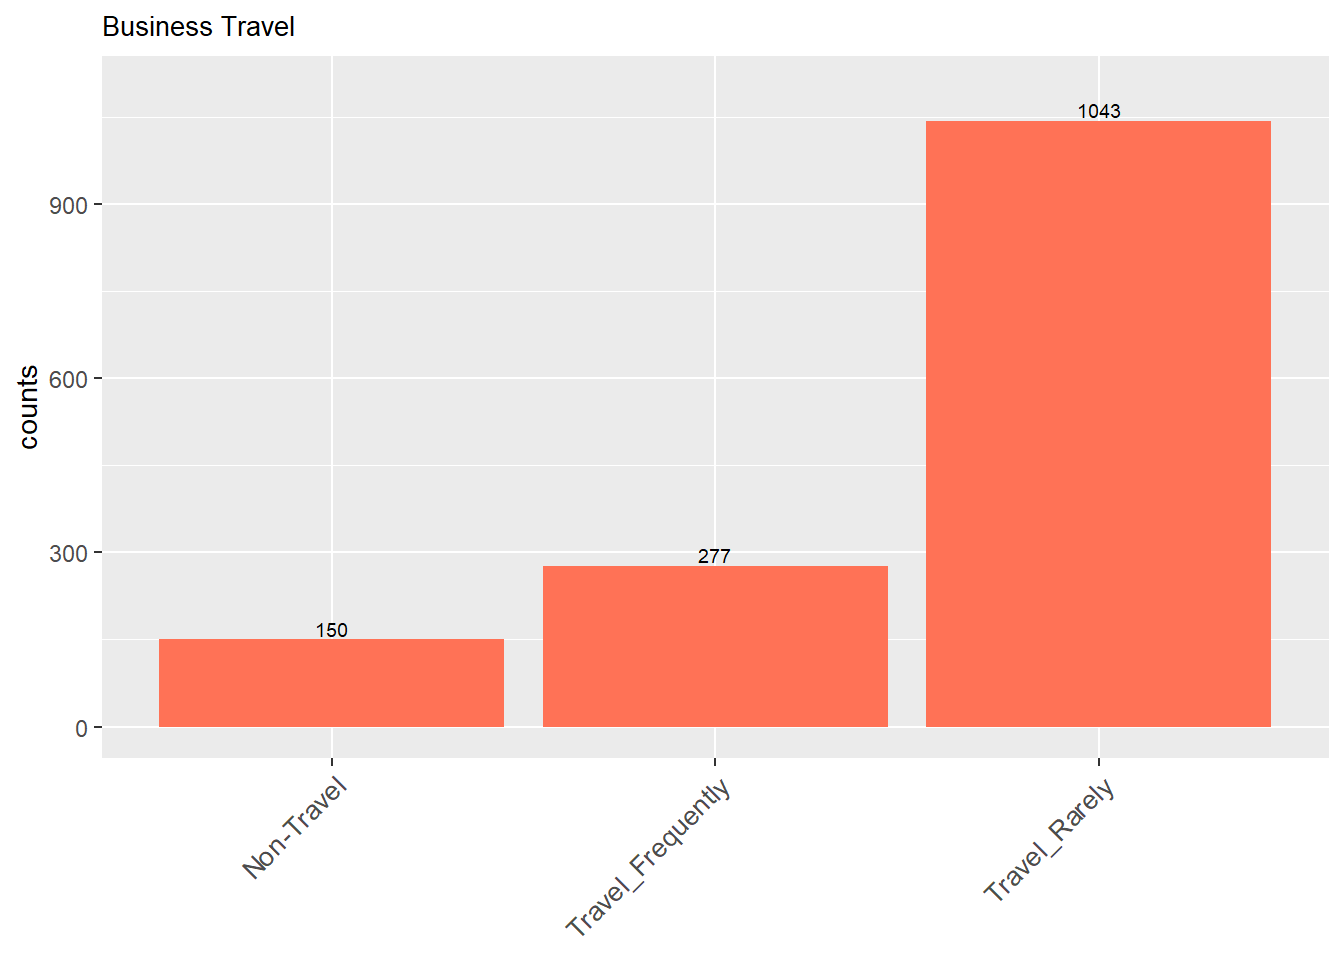
\includegraphics{DDSAnalytics_Case_Study_files/figure-latex/uni_cat_demo_work-1.pdf}

\subsubsection{Observations}\label{observations-4}

\begin{itemize}
\tightlist
\item
  Approximately 71\% of the employees rarely travel for work.
\item
  Approximately 30\% of the employees rate environment satisfaction as
  high or very high.
\item
  Approximately 59\% of the employees rated their job involvement at
  work as high.
\item
  Approximately 30\% of the employees rate job satisfaction as high or
  very high.
\item
  Approximately 72\% of the employees do not work overtime.
\item
  Approximately 85\% of the employees have an Excellent Performance
  Rating.
\item
  More than half (65\%) of the employees work in Research \&
  Development.
\item
  Most employees work as Sales Executives, Research Scientists or
  Laboratory Technicians
\end{itemize}

\begin{center}\rule{0.5\linewidth}{\linethickness}\end{center}

\section{Bivariate EDA}\label{bivariate-eda}

Now start analyzing data in relation to our attrition variable. Since
attribution is the target variable we want to see if we uncover any
hidden relationships. As before start with the non-categorical (numeric)
variables first and then move to the categorical variables.

\subsection{Non-Categorical
Variables}\label{non-categorical-variables-1}

\subsubsection{Employee Demographics -
Basic}\label{employee-demographics---basic-1}

\begin{Shaded}
\begin{Highlighting}[]
\CommentTok{#Evaluate non-categorical variables as they relate to the attrition variable. We'll use density plots with alpha = 0.5}
\CommentTok{#Age}
\NormalTok{p1 =}\StringTok{ }\NormalTok{empDF }\OperatorTok
\StringTok{  }\KeywordTok{ggplot}\NormalTok{(}\KeywordTok{aes}\NormalTok{(}\DataTypeTok{x =}\NormalTok{ Age, }\DataTypeTok{fill =}\NormalTok{ Attrition)) }\OperatorTok{+}\StringTok{ }\KeywordTok{geom_density}\NormalTok{(}\DataTypeTok{alpha =} \FloatTok{0.5}\NormalTok{) }\OperatorTok{+}\StringTok{ }\KeywordTok{ggtitle}\NormalTok{(}\StringTok{"Age"}\NormalTok{) }\OperatorTok{+}\StringTok{ }\KeywordTok{theme}\NormalTok{(}\DataTypeTok{plot.title =} \KeywordTok{element_text}\NormalTok{(}\DataTypeTok{size =}\DecValTok{10}\NormalTok{),}\DataTypeTok{axis.text.x =} \KeywordTok{element_text}\NormalTok{(}\DataTypeTok{size =}\DecValTok{7}\NormalTok{,}\DataTypeTok{angle =} \DecValTok{45}\NormalTok{, }\DataTypeTok{hjust =} \DecValTok{1}\NormalTok{),}\DataTypeTok{axis.title.x=}\KeywordTok{element_blank}\NormalTok{())}

\CommentTok{#Distance from Home}
\NormalTok{p2 =}\StringTok{ }\NormalTok{empDF }\OperatorTok
\StringTok{  }\KeywordTok{ggplot}\NormalTok{(}\KeywordTok{aes}\NormalTok{(}\DataTypeTok{x =}\NormalTok{ DistanceFromHome, }\DataTypeTok{fill =}\NormalTok{ Attrition)) }\OperatorTok{+}\StringTok{ }\KeywordTok{geom_density}\NormalTok{(}\DataTypeTok{alpha =} \FloatTok{0.5}\NormalTok{) }\OperatorTok{+}\StringTok{ }\KeywordTok{ggtitle}\NormalTok{(}\StringTok{"Distance From Home"}\NormalTok{)  }\OperatorTok{+}\StringTok{ }\KeywordTok{theme}\NormalTok{(}\DataTypeTok{plot.title =} \KeywordTok{element_text}\NormalTok{(}\DataTypeTok{size =}\DecValTok{10}\NormalTok{),}\DataTypeTok{axis.text.x =} \KeywordTok{element_text}\NormalTok{(}\DataTypeTok{size =}\DecValTok{7}\NormalTok{,}\DataTypeTok{angle =} \DecValTok{45}\NormalTok{, }\DataTypeTok{hjust =} \DecValTok{1}\NormalTok{),}\DataTypeTok{axis.title.x=}\KeywordTok{element_blank}\NormalTok{())}

\CommentTok{#Number of Companies Worked}
\NormalTok{p3 =}\StringTok{ }\NormalTok{empDF }\OperatorTok
\StringTok{  }\KeywordTok{ggplot}\NormalTok{(}\KeywordTok{aes}\NormalTok{(}\DataTypeTok{x =}\NormalTok{ NumCompaniesWorked, }\DataTypeTok{fill =}\NormalTok{ Attrition)) }\OperatorTok{+}\StringTok{ }\KeywordTok{geom_density}\NormalTok{(}\DataTypeTok{alpha =} \FloatTok{0.5}\NormalTok{) }\OperatorTok{+}\StringTok{ }\KeywordTok{ggtitle}\NormalTok{(}\StringTok{"Number of Companies"}\NormalTok{)  }\OperatorTok{+}\StringTok{ }\KeywordTok{theme}\NormalTok{(}\DataTypeTok{plot.title =} \KeywordTok{element_text}\NormalTok{(}\DataTypeTok{size =}\DecValTok{10}\NormalTok{),}\DataTypeTok{axis.text.x =} \KeywordTok{element_text}\NormalTok{(}\DataTypeTok{size =}\DecValTok{7}\NormalTok{,}\DataTypeTok{angle =} \DecValTok{45}\NormalTok{, }\DataTypeTok{hjust =} \DecValTok{1}\NormalTok{),}\DataTypeTok{axis.title.x=}\KeywordTok{element_blank}\NormalTok{())}

\CommentTok{#Total Working Years}
\NormalTok{p4 =}\StringTok{ }\NormalTok{empDF }\OperatorTok
\StringTok{  }\KeywordTok{ggplot}\NormalTok{(}\KeywordTok{aes}\NormalTok{(}\DataTypeTok{x =}\NormalTok{ TotalWorkingYears, }\DataTypeTok{fill =}\NormalTok{ Attrition)) }\OperatorTok{+}\StringTok{ }\KeywordTok{geom_density}\NormalTok{(}\DataTypeTok{alpha =} \FloatTok{0.5}\NormalTok{) }\OperatorTok{+}\StringTok{ }\KeywordTok{ggtitle}\NormalTok{(}\StringTok{"Total Working Years"}\NormalTok{)  }\OperatorTok{+}\StringTok{ }\KeywordTok{theme}\NormalTok{(}\DataTypeTok{plot.title =} \KeywordTok{element_text}\NormalTok{(}\DataTypeTok{size =}\DecValTok{10}\NormalTok{),}\DataTypeTok{axis.text.x =} \KeywordTok{element_text}\NormalTok{(}\DataTypeTok{size =}\DecValTok{7}\NormalTok{,}\DataTypeTok{angle =} \DecValTok{45}\NormalTok{, }\DataTypeTok{hjust =} \DecValTok{1}\NormalTok{),}\DataTypeTok{axis.title.x=}\KeywordTok{element_blank}\NormalTok{())}

\KeywordTok{ggarrange}\NormalTok{(p1,p2,p3,p4)}
\end{Highlighting}
\end{Shaded}

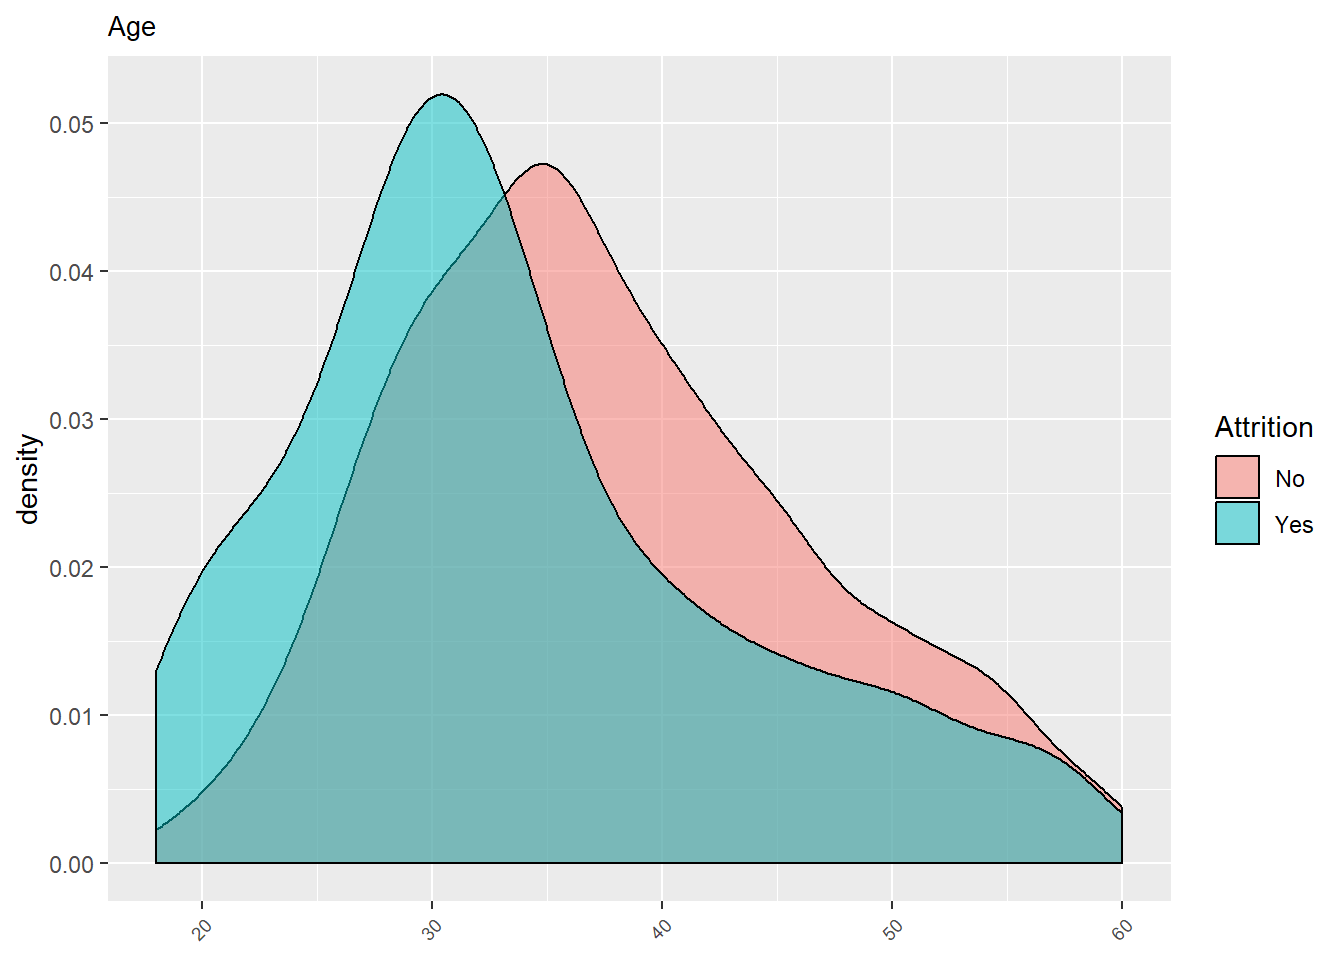
\includegraphics{DDSAnalytics_Case_Study_files/figure-latex/biv_non_cat_basic-1.pdf}

\subsubsection{Observations}\label{observations-5}

\begin{itemize}
\tightlist
\item
  Younger employees between 25-35 years have a higher attrition rate.
\item
  There is a higher attrition rate when the distance from home is
  greater than 10. Attrition rate is less below 10.
\item
  Attrition rate seems to be higher for employees who have work with 5
  to 7 companies.
\item
  The highest attrition rates seem to be with employees with between 0
  to 7 years of work experience.
\end{itemize}

\subsubsection{Employee Demographics -
Financial}\label{employee-demographics---financial-1}

\begin{Shaded}
\begin{Highlighting}[]
\CommentTok{#Evaluate non-categorical variables as they relate to the attrition variable for financial values. We'll use density plots with alpha = 0.5}
\CommentTok{#Hourly Rate}
\NormalTok{p1 =}\StringTok{ }\NormalTok{empDF }\OperatorTok
\StringTok{  }\KeywordTok{ggplot}\NormalTok{(}\KeywordTok{aes}\NormalTok{(}\DataTypeTok{x =}\NormalTok{ HourlyRate, }\DataTypeTok{fill =}\NormalTok{ Attrition)) }\OperatorTok{+}\StringTok{ }\KeywordTok{geom_density}\NormalTok{(}\DataTypeTok{alpha =} \FloatTok{0.5}\NormalTok{) }\OperatorTok{+}\StringTok{ }\KeywordTok{ggtitle}\NormalTok{(}\StringTok{"Hourly Rate"}\NormalTok{) }\OperatorTok{+}\StringTok{ }\KeywordTok{theme}\NormalTok{(}\DataTypeTok{plot.title =} \KeywordTok{element_text}\NormalTok{(}\DataTypeTok{size =}\DecValTok{10}\NormalTok{),}\DataTypeTok{axis.text.x =} \KeywordTok{element_text}\NormalTok{(}\DataTypeTok{size =}\DecValTok{7}\NormalTok{,}\DataTypeTok{angle =} \DecValTok{45}\NormalTok{, }\DataTypeTok{hjust =} \DecValTok{1}\NormalTok{),}\DataTypeTok{axis.title.x=}\KeywordTok{element_blank}\NormalTok{())}

\CommentTok{#Daily Rate}
\NormalTok{p2 =}\StringTok{ }\NormalTok{empDF }\OperatorTok
\StringTok{  }\KeywordTok{ggplot}\NormalTok{(}\KeywordTok{aes}\NormalTok{(}\DataTypeTok{x =}\NormalTok{ DailyRate, }\DataTypeTok{fill =}\NormalTok{ Attrition)) }\OperatorTok{+}\StringTok{ }\KeywordTok{geom_density}\NormalTok{(}\DataTypeTok{alpha =} \FloatTok{0.5}\NormalTok{) }\OperatorTok{+}\StringTok{ }\KeywordTok{ggtitle}\NormalTok{(}\StringTok{"Daily Rate"}\NormalTok{) }\OperatorTok{+}\StringTok{ }\KeywordTok{theme}\NormalTok{(}\DataTypeTok{plot.title =} \KeywordTok{element_text}\NormalTok{(}\DataTypeTok{size =}\DecValTok{10}\NormalTok{),}\DataTypeTok{axis.text.x =} \KeywordTok{element_text}\NormalTok{(}\DataTypeTok{size =}\DecValTok{7}\NormalTok{,}\DataTypeTok{angle =} \DecValTok{45}\NormalTok{, }\DataTypeTok{hjust =} \DecValTok{1}\NormalTok{),}\DataTypeTok{axis.title.x=}\KeywordTok{element_blank}\NormalTok{())}

\CommentTok{#Monthly Rate}
\NormalTok{p3 =}\StringTok{ }\NormalTok{empDF }\OperatorTok
\StringTok{  }\KeywordTok{ggplot}\NormalTok{(}\KeywordTok{aes}\NormalTok{(}\DataTypeTok{x =}\NormalTok{ MonthlyRate, }\DataTypeTok{fill =}\NormalTok{ Attrition)) }\OperatorTok{+}\StringTok{ }\KeywordTok{geom_density}\NormalTok{(}\DataTypeTok{alpha =} \FloatTok{0.5}\NormalTok{)}\OperatorTok{+}\StringTok{ }\KeywordTok{ggtitle}\NormalTok{(}\StringTok{"Monthly Rate"}\NormalTok{) }\OperatorTok{+}\StringTok{ }\KeywordTok{theme}\NormalTok{(}\DataTypeTok{plot.title =} \KeywordTok{element_text}\NormalTok{(}\DataTypeTok{size =}\DecValTok{10}\NormalTok{),}\DataTypeTok{axis.text.x =} \KeywordTok{element_text}\NormalTok{(}\DataTypeTok{size =}\DecValTok{7}\NormalTok{,}\DataTypeTok{angle =} \DecValTok{45}\NormalTok{, }\DataTypeTok{hjust =} \DecValTok{1}\NormalTok{),}\DataTypeTok{axis.title.x=}\KeywordTok{element_blank}\NormalTok{())}

\KeywordTok{ggarrange}\NormalTok{(p1,p2,p3)}
\end{Highlighting}
\end{Shaded}

\includegraphics{DDSAnalytics_Case_Study_files/figure-latex/biv_non_cat_financial-1.pdf}

\subsubsection{Observations}\label{observations-6}

\begin{itemize}
\tightlist
\item
  There are no observable patterns in this data.
\end{itemize}

\subsubsection{Employee Demographics - Work
Environment}\label{employee-demographics---work-environment-2}

\begin{Shaded}
\begin{Highlighting}[]
\CommentTok{#Evaluate non-categorical variables as they relate to the attrition variable for work environment values. We'll use density plots with alpha = 0.5}
\CommentTok{#Monthly Income}
\NormalTok{p1 =}\StringTok{ }\NormalTok{empDF }\OperatorTok
\StringTok{  }\KeywordTok{ggplot}\NormalTok{(}\KeywordTok{aes}\NormalTok{(}\DataTypeTok{x =}\NormalTok{ MonthlyIncome, }\DataTypeTok{fill =}\NormalTok{ Attrition)) }\OperatorTok{+}\StringTok{ }\KeywordTok{geom_density}\NormalTok{(}\DataTypeTok{alpha =} \FloatTok{0.5}\NormalTok{) }\OperatorTok{+}\StringTok{ }\KeywordTok{ggtitle}\NormalTok{(}\StringTok{"Monthly Income"}\NormalTok{) }\OperatorTok{+}\StringTok{ }\KeywordTok{theme}\NormalTok{(}\DataTypeTok{plot.title =} \KeywordTok{element_text}\NormalTok{(}\DataTypeTok{size =}\DecValTok{10}\NormalTok{),}\DataTypeTok{axis.text.x =} \KeywordTok{element_text}\NormalTok{(}\DataTypeTok{size =}\DecValTok{7}\NormalTok{,}\DataTypeTok{angle =} \DecValTok{45}\NormalTok{, }\DataTypeTok{hjust =} \DecValTok{1}\NormalTok{),}\DataTypeTok{axis.title.x=}\KeywordTok{element_blank}\NormalTok{())}

\CommentTok{#Salary Hike}
\NormalTok{p2 =}\StringTok{ }\NormalTok{empDF }\OperatorTok
\StringTok{  }\KeywordTok{ggplot}\NormalTok{(}\KeywordTok{aes}\NormalTok{(}\DataTypeTok{x =}\NormalTok{ PercentSalaryHike, }\DataTypeTok{fill =}\NormalTok{ Attrition)) }\OperatorTok{+}\StringTok{ }\KeywordTok{geom_density}\NormalTok{(}\DataTypeTok{alpha =} \FloatTok{0.5}\NormalTok{) }\OperatorTok{+}\StringTok{ }\KeywordTok{ggtitle}\NormalTok{(}\StringTok{"Percentage Salary Hike"}\NormalTok{) }\OperatorTok{+}\StringTok{ }\KeywordTok{theme}\NormalTok{(}\DataTypeTok{plot.title =} \KeywordTok{element_text}\NormalTok{(}\DataTypeTok{size =}\DecValTok{10}\NormalTok{),}\DataTypeTok{axis.text.x =} \KeywordTok{element_text}\NormalTok{(}\DataTypeTok{size =}\DecValTok{7}\NormalTok{,}\DataTypeTok{angle =} \DecValTok{45}\NormalTok{, }\DataTypeTok{hjust =} \DecValTok{1}\NormalTok{),}\DataTypeTok{axis.title.x=}\KeywordTok{element_blank}\NormalTok{())}

\CommentTok{#Years at Company}
\NormalTok{p3 =}\StringTok{ }\NormalTok{empDF }\OperatorTok
\StringTok{  }\KeywordTok{ggplot}\NormalTok{(}\KeywordTok{aes}\NormalTok{(}\DataTypeTok{x =}\NormalTok{ YearsAtCompany, }\DataTypeTok{fill =}\NormalTok{ Attrition)) }\OperatorTok{+}\StringTok{ }\KeywordTok{geom_density}\NormalTok{(}\DataTypeTok{alpha =} \FloatTok{0.5}\NormalTok{) }\OperatorTok{+}\StringTok{ }\KeywordTok{ggtitle}\NormalTok{(}\StringTok{"Years At Company"}\NormalTok{) }\OperatorTok{+}\StringTok{ }\KeywordTok{theme}\NormalTok{(}\DataTypeTok{plot.title =} \KeywordTok{element_text}\NormalTok{(}\DataTypeTok{size =}\DecValTok{10}\NormalTok{),}\DataTypeTok{axis.text.x =} \KeywordTok{element_text}\NormalTok{(}\DataTypeTok{size =}\DecValTok{7}\NormalTok{,}\DataTypeTok{angle =} \DecValTok{45}\NormalTok{, }\DataTypeTok{hjust =} \DecValTok{1}\NormalTok{),}\DataTypeTok{axis.title.x=}\KeywordTok{element_blank}\NormalTok{())}

\CommentTok{#Years In Role}
\NormalTok{p4 =}\StringTok{ }\NormalTok{empDF }\OperatorTok
\StringTok{  }\KeywordTok{ggplot}\NormalTok{(}\KeywordTok{aes}\NormalTok{(}\DataTypeTok{x =}\NormalTok{ YearsInCurrentRole, }\DataTypeTok{fill =}\NormalTok{ Attrition)) }\OperatorTok{+}\StringTok{ }\KeywordTok{geom_density}\NormalTok{(}\DataTypeTok{alpha =} \FloatTok{0.5}\NormalTok{) }\OperatorTok{+}\StringTok{ }\KeywordTok{ggtitle}\NormalTok{(}\StringTok{"Years in Current Role"}\NormalTok{) }\OperatorTok{+}\StringTok{ }\KeywordTok{theme}\NormalTok{(}\DataTypeTok{plot.title =} \KeywordTok{element_text}\NormalTok{(}\DataTypeTok{size =}\DecValTok{10}\NormalTok{),}\DataTypeTok{axis.text.x =} \KeywordTok{element_text}\NormalTok{(}\DataTypeTok{size =}\DecValTok{7}\NormalTok{,}\DataTypeTok{angle =} \DecValTok{45}\NormalTok{, }\DataTypeTok{hjust =} \DecValTok{1}\NormalTok{),}\DataTypeTok{axis.title.x=}\KeywordTok{element_blank}\NormalTok{())}

\CommentTok{#Years Since Promotion}
\NormalTok{p5 =}\StringTok{ }\NormalTok{empDF }\OperatorTok
\StringTok{  }\KeywordTok{ggplot}\NormalTok{(}\KeywordTok{aes}\NormalTok{(}\DataTypeTok{x =}\NormalTok{ YearsSinceLastPromotion, }\DataTypeTok{fill =}\NormalTok{ Attrition)) }\OperatorTok{+}\StringTok{ }\KeywordTok{geom_density}\NormalTok{(}\DataTypeTok{alpha =} \FloatTok{0.5}\NormalTok{) }\OperatorTok{+}\StringTok{ }\KeywordTok{ggtitle}\NormalTok{(}\StringTok{"Years Since Last Promotion"}\NormalTok{) }\OperatorTok{+}\StringTok{ }\KeywordTok{theme}\NormalTok{(}\DataTypeTok{plot.title =} \KeywordTok{element_text}\NormalTok{(}\DataTypeTok{size =}\DecValTok{10}\NormalTok{),}\DataTypeTok{axis.text.x =} \KeywordTok{element_text}\NormalTok{(}\DataTypeTok{size =}\DecValTok{7}\NormalTok{,}\DataTypeTok{angle =} \DecValTok{45}\NormalTok{, }\DataTypeTok{hjust =} \DecValTok{1}\NormalTok{),}\DataTypeTok{axis.title.x=}\KeywordTok{element_blank}\NormalTok{())}

\CommentTok{#Years with Current Manager}
\NormalTok{p6 =}\StringTok{ }\NormalTok{empDF }\OperatorTok
\StringTok{  }\KeywordTok{ggplot}\NormalTok{(}\KeywordTok{aes}\NormalTok{(}\DataTypeTok{x =}\NormalTok{ YearsWithCurrManager, }\DataTypeTok{fill =}\NormalTok{ Attrition)) }\OperatorTok{+}\StringTok{ }\KeywordTok{geom_density}\NormalTok{(}\DataTypeTok{alpha =} \FloatTok{0.5}\NormalTok{) }\OperatorTok{+}\StringTok{ }\KeywordTok{ggtitle}\NormalTok{(}\StringTok{"Years With Current Manager"}\NormalTok{) }\OperatorTok{+}\StringTok{ }\KeywordTok{theme}\NormalTok{(}\DataTypeTok{plot.title =} \KeywordTok{element_text}\NormalTok{(}\DataTypeTok{size =}\DecValTok{10}\NormalTok{),}\DataTypeTok{axis.text.x =} \KeywordTok{element_text}\NormalTok{(}\DataTypeTok{size =}\DecValTok{7}\NormalTok{,}\DataTypeTok{angle =} \DecValTok{45}\NormalTok{, }\DataTypeTok{hjust =} \DecValTok{1}\NormalTok{),}\DataTypeTok{axis.title.x=}\KeywordTok{element_blank}\NormalTok{())}

\KeywordTok{ggarrange}\NormalTok{(p1,p2,p3,p4,p5,p6, }\DataTypeTok{ncol=}\DecValTok{2}\NormalTok{, }\DataTypeTok{nrow=}\DecValTok{3}\NormalTok{)}
\end{Highlighting}
\end{Shaded}

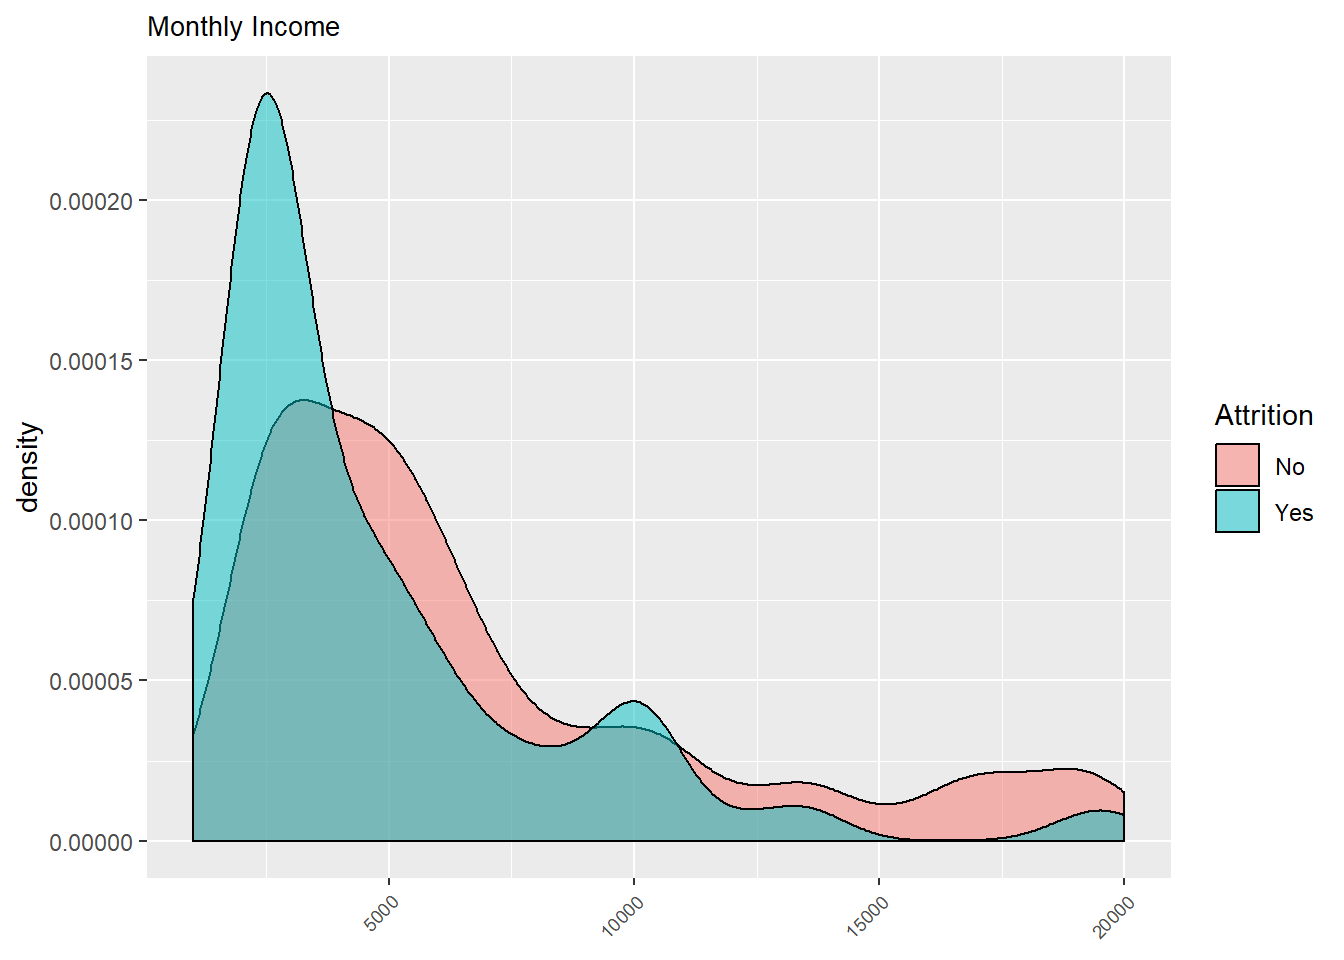
\includegraphics{DDSAnalytics_Case_Study_files/figure-latex/biv_non_cat_work-1.pdf}

\subsubsection{Observations}\label{observations-7}

\begin{itemize}
\tightlist
\item
  Peak attrition occurs when the monthly income rate is about \$2500.
\item
  Peak attrition rate also occurs when the employee is with the company
  for approximately 0-2 years.
\item
  Attrition rate is higher when the employee is in the same role for 0-2
  years or 6 years approximately, based off of the bi-modal nature of
  the graph.
\item
  Attrition rate is higher when the employee is with the same manager
  for less than 1.5 yeas or 6 years approximately, based off of the
  bi-modal nature of the graph.
\end{itemize}

\subsection{Bivariate EDA - Categorical
Variables}\label{bivariate-eda---categorical-variables}

\subsubsection{Employee Demographics -
Personal}\label{employee-demographics---personal-1}

\begin{Shaded}
\begin{Highlighting}[]
\CommentTok{#Investigate categorical variables as they relate to the attrition variable. Focus on the personal variables in this section}
\CommentTok{#Gender}
\NormalTok{p1 =}\StringTok{ }\NormalTok{empDF }\OperatorTok
\StringTok{  }\KeywordTok{group_by}\NormalTok{(Gender) }\OperatorTok
\StringTok{  }\NormalTok{dplyr}\OperatorTok{::}\KeywordTok{summarise}\NormalTok{(}\DataTypeTok{attrition_rate =} \KeywordTok{round}\NormalTok{((}\KeywordTok{sum}\NormalTok{(}\KeywordTok{if_else}\NormalTok{(Attrition }\OperatorTok{==}\StringTok{ "Yes"}\NormalTok{,}\DecValTok{1}\NormalTok{,}\DecValTok{0}\NormalTok{))}\OperatorTok{/}\KeywordTok{n}\NormalTok{()}\OperatorTok{*}\DecValTok{100}\NormalTok{),}\DecValTok{2}\NormalTok{)) }\OperatorTok
\StringTok{  }\KeywordTok{ggplot}\NormalTok{(}\KeywordTok{aes}\NormalTok{(}\DataTypeTok{x =}\NormalTok{ Gender, }\DataTypeTok{y =}\NormalTok{ attrition_rate))}\OperatorTok{+}\StringTok{ }\KeywordTok{geom_bar}\NormalTok{(}\DataTypeTok{stat =} \StringTok{'identity'}\NormalTok{,}\DataTypeTok{fill =} \StringTok{"blue"}\NormalTok{) }\OperatorTok{+}\StringTok{ }\KeywordTok{ggtitle}\NormalTok{(}\StringTok{"Attrition Rate - Gender"}\NormalTok{) }\OperatorTok{+}\StringTok{ }\KeywordTok{theme}\NormalTok{(}\DataTypeTok{plot.title =} \KeywordTok{element_text}\NormalTok{(}\DataTypeTok{size =}\DecValTok{10}\NormalTok{),}\DataTypeTok{axis.text.x =} \KeywordTok{element_text}\NormalTok{(}\DataTypeTok{size =}\DecValTok{7}\NormalTok{,}\DataTypeTok{angle =} \DecValTok{45}\NormalTok{, }\DataTypeTok{hjust =} \DecValTok{1}\NormalTok{),}\DataTypeTok{axis.title.x=}\KeywordTok{element_blank}\NormalTok{()) }\OperatorTok{+}\KeywordTok{geom_text}\NormalTok{(}\KeywordTok{aes}\NormalTok{(}\DataTypeTok{label=}\NormalTok{attrition_rate), }\DataTypeTok{size =} \FloatTok{2.5}\NormalTok{, }\DataTypeTok{position=}\KeywordTok{position_dodge}\NormalTok{(}\DataTypeTok{width=}\FloatTok{0.2}\NormalTok{), }\DataTypeTok{vjust=}\OperatorTok{-}\FloatTok{0.25}\NormalTok{)}\OperatorTok{+}\StringTok{ }\KeywordTok{scale_y_continuous}\NormalTok{(}\DataTypeTok{limits =} \KeywordTok{c}\NormalTok{(}\DecValTok{0}\NormalTok{, }\DecValTok{20}\NormalTok{))}

\CommentTok{#Education}
\NormalTok{p2 =}\StringTok{ }\NormalTok{empDF }\OperatorTok
\StringTok{  }\KeywordTok{group_by}\NormalTok{(Education) }\OperatorTok
\StringTok{  }\NormalTok{dplyr}\OperatorTok{::}\KeywordTok{summarise}\NormalTok{(}\DataTypeTok{attrition_rate =} \KeywordTok{round}\NormalTok{((}\KeywordTok{sum}\NormalTok{(}\KeywordTok{if_else}\NormalTok{(Attrition }\OperatorTok{==}\StringTok{ "Yes"}\NormalTok{,}\DecValTok{1}\NormalTok{,}\DecValTok{0}\NormalTok{))}\OperatorTok{/}\KeywordTok{n}\NormalTok{()}\OperatorTok{*}\DecValTok{100}\NormalTok{),}\DecValTok{2}\NormalTok{)) }\OperatorTok
\StringTok{  }\KeywordTok{ggplot}\NormalTok{(}\KeywordTok{aes}\NormalTok{(}\DataTypeTok{x =}\NormalTok{ Education, }\DataTypeTok{y =}\NormalTok{ attrition_rate))}\OperatorTok{+}\StringTok{ }\KeywordTok{geom_bar}\NormalTok{(}\DataTypeTok{stat =} \StringTok{'identity'}\NormalTok{,}\DataTypeTok{fill =} \StringTok{"blue"}\NormalTok{) }\OperatorTok{+}\StringTok{ }\KeywordTok{ggtitle}\NormalTok{(}\StringTok{"Attrition Rate - Education"}\NormalTok{) }\OperatorTok{+}\StringTok{ }\KeywordTok{theme}\NormalTok{(}\DataTypeTok{plot.title =} \KeywordTok{element_text}\NormalTok{(}\DataTypeTok{size =}\DecValTok{10}\NormalTok{),}\DataTypeTok{axis.text.x =} \KeywordTok{element_text}\NormalTok{(}\DataTypeTok{size =}\DecValTok{7}\NormalTok{,}\DataTypeTok{angle =} \DecValTok{45}\NormalTok{, }\DataTypeTok{hjust =} \DecValTok{1}\NormalTok{),}\DataTypeTok{axis.title.x=}\KeywordTok{element_blank}\NormalTok{()) }\OperatorTok{+}\KeywordTok{geom_text}\NormalTok{(}\KeywordTok{aes}\NormalTok{(}\DataTypeTok{label=}\NormalTok{attrition_rate), }\DataTypeTok{size =} \FloatTok{2.5}\NormalTok{, }\DataTypeTok{position=}\KeywordTok{position_dodge}\NormalTok{(}\DataTypeTok{width=}\FloatTok{0.2}\NormalTok{), }\DataTypeTok{vjust=}\OperatorTok{-}\FloatTok{0.25}\NormalTok{)}\OperatorTok{+}\StringTok{ }\KeywordTok{scale_y_continuous}\NormalTok{(}\DataTypeTok{limits =} \KeywordTok{c}\NormalTok{(}\DecValTok{0}\NormalTok{, }\DecValTok{20}\NormalTok{))}

\CommentTok{#Education Field}
\NormalTok{p3 =}\StringTok{ }\NormalTok{empDF }\OperatorTok
\StringTok{  }\KeywordTok{group_by}\NormalTok{(EducationField) }\OperatorTok
\StringTok{  }\NormalTok{dplyr}\OperatorTok{::}\KeywordTok{summarise}\NormalTok{(}\DataTypeTok{attrition_rate =} \KeywordTok{round}\NormalTok{((}\KeywordTok{sum}\NormalTok{(}\KeywordTok{if_else}\NormalTok{(Attrition }\OperatorTok{==}\StringTok{ "Yes"}\NormalTok{,}\DecValTok{1}\NormalTok{,}\DecValTok{0}\NormalTok{))}\OperatorTok{/}\KeywordTok{n}\NormalTok{()}\OperatorTok{*}\DecValTok{100}\NormalTok{),}\DecValTok{2}\NormalTok{)) }\OperatorTok
\StringTok{  }\KeywordTok{ggplot}\NormalTok{(}\KeywordTok{aes}\NormalTok{(}\DataTypeTok{x =}\NormalTok{ EducationField, }\DataTypeTok{y =}\NormalTok{ attrition_rate))}\OperatorTok{+}\StringTok{ }\KeywordTok{geom_bar}\NormalTok{(}\DataTypeTok{stat =} \StringTok{'identity'}\NormalTok{,}\DataTypeTok{fill =} \StringTok{"blue"}\NormalTok{) }\OperatorTok{+}\StringTok{ }\KeywordTok{ggtitle}\NormalTok{(}\StringTok{"Attrition Rate - Education Field"}\NormalTok{) }\OperatorTok{+}\StringTok{ }\KeywordTok{theme}\NormalTok{(}\DataTypeTok{plot.title =} \KeywordTok{element_text}\NormalTok{(}\DataTypeTok{size =}\DecValTok{10}\NormalTok{),}\DataTypeTok{axis.text.x =} \KeywordTok{element_text}\NormalTok{(}\DataTypeTok{size =}\DecValTok{7}\NormalTok{,}\DataTypeTok{angle =} \DecValTok{45}\NormalTok{, }\DataTypeTok{hjust =} \DecValTok{1}\NormalTok{),}\DataTypeTok{axis.title.x=}\KeywordTok{element_blank}\NormalTok{()) }\OperatorTok{+}\KeywordTok{geom_text}\NormalTok{(}\KeywordTok{aes}\NormalTok{(}\DataTypeTok{label=}\NormalTok{attrition_rate), }\DataTypeTok{size =} \FloatTok{2.5}\NormalTok{, }\DataTypeTok{position=}\KeywordTok{position_dodge}\NormalTok{(}\DataTypeTok{width=}\FloatTok{0.2}\NormalTok{), }\DataTypeTok{vjust=}\OperatorTok{-}\FloatTok{0.25}\NormalTok{)}\OperatorTok{+}\StringTok{ }\KeywordTok{scale_y_continuous}\NormalTok{(}\DataTypeTok{limits =} \KeywordTok{c}\NormalTok{(}\DecValTok{0}\NormalTok{, }\DecValTok{30}\NormalTok{))}

\CommentTok{#Marital Status}
\NormalTok{p4 =}\StringTok{ }\NormalTok{empDF }\OperatorTok
\StringTok{  }\KeywordTok{group_by}\NormalTok{(MaritalStatus) }\OperatorTok
\StringTok{  }\NormalTok{dplyr}\OperatorTok{::}\KeywordTok{summarise}\NormalTok{(}\DataTypeTok{attrition_rate =} \KeywordTok{round}\NormalTok{((}\KeywordTok{sum}\NormalTok{(}\KeywordTok{if_else}\NormalTok{(Attrition }\OperatorTok{==}\StringTok{ "Yes"}\NormalTok{,}\DecValTok{1}\NormalTok{,}\DecValTok{0}\NormalTok{))}\OperatorTok{/}\KeywordTok{n}\NormalTok{()}\OperatorTok{*}\DecValTok{100}\NormalTok{),}\DecValTok{2}\NormalTok{)) }\OperatorTok
\StringTok{  }\KeywordTok{ggplot}\NormalTok{(}\KeywordTok{aes}\NormalTok{(}\DataTypeTok{x =}\NormalTok{ MaritalStatus, }\DataTypeTok{y =}\NormalTok{ attrition_rate))}\OperatorTok{+}\StringTok{ }\KeywordTok{geom_bar}\NormalTok{(}\DataTypeTok{stat =} \StringTok{'identity'}\NormalTok{,}\DataTypeTok{fill =} \StringTok{"blue"}\NormalTok{) }\OperatorTok{+}\StringTok{ }\KeywordTok{ggtitle}\NormalTok{(}\StringTok{"Attrition Rate - Marital Status"}\NormalTok{) }\OperatorTok{+}\StringTok{ }\KeywordTok{theme}\NormalTok{(}\DataTypeTok{plot.title =} \KeywordTok{element_text}\NormalTok{(}\DataTypeTok{size =}\DecValTok{10}\NormalTok{),}\DataTypeTok{axis.text.x =} \KeywordTok{element_text}\NormalTok{(}\DataTypeTok{size =}\DecValTok{7}\NormalTok{,}\DataTypeTok{angle =} \DecValTok{45}\NormalTok{, }\DataTypeTok{hjust =} \DecValTok{1}\NormalTok{),}\DataTypeTok{axis.title.x=}\KeywordTok{element_blank}\NormalTok{()) }\OperatorTok{+}\KeywordTok{geom_text}\NormalTok{(}\KeywordTok{aes}\NormalTok{(}\DataTypeTok{label=}\NormalTok{attrition_rate), }\DataTypeTok{size =} \FloatTok{2.5}\NormalTok{, }\DataTypeTok{position=}\KeywordTok{position_dodge}\NormalTok{(}\DataTypeTok{width=}\FloatTok{0.2}\NormalTok{), }\DataTypeTok{vjust=}\OperatorTok{-}\FloatTok{0.25}\NormalTok{)}\OperatorTok{+}\StringTok{ }\KeywordTok{scale_y_continuous}\NormalTok{(}\DataTypeTok{limits =} \KeywordTok{c}\NormalTok{(}\DecValTok{0}\NormalTok{, }\DecValTok{30}\NormalTok{))}

\CommentTok{#Relationship Satisfaction}
\NormalTok{p5 =}\StringTok{ }\NormalTok{empDF }\OperatorTok
\StringTok{  }\KeywordTok{group_by}\NormalTok{(RelationshipSatisfaction) }\OperatorTok
\StringTok{  }\NormalTok{dplyr}\OperatorTok{::}\KeywordTok{summarise}\NormalTok{(}\DataTypeTok{attrition_rate =} \KeywordTok{round}\NormalTok{((}\KeywordTok{sum}\NormalTok{(}\KeywordTok{if_else}\NormalTok{(Attrition }\OperatorTok{==}\StringTok{ "Yes"}\NormalTok{,}\DecValTok{1}\NormalTok{,}\DecValTok{0}\NormalTok{))}\OperatorTok{/}\KeywordTok{n}\NormalTok{()}\OperatorTok{*}\DecValTok{100}\NormalTok{),}\DecValTok{2}\NormalTok{)) }\OperatorTok
\StringTok{  }\KeywordTok{ggplot}\NormalTok{(}\KeywordTok{aes}\NormalTok{(}\DataTypeTok{x =} \KeywordTok{as.factor}\NormalTok{(RelationshipSatisfaction), }\DataTypeTok{y =}\NormalTok{ attrition_rate))}\OperatorTok{+}\StringTok{ }\KeywordTok{geom_bar}\NormalTok{(}\DataTypeTok{stat =} \StringTok{'identity'}\NormalTok{,}\DataTypeTok{fill =} \StringTok{"blue"}\NormalTok{) }\OperatorTok{+}\StringTok{ }\KeywordTok{ggtitle}\NormalTok{(}\StringTok{"Attrition Rate - Relationship Satisfaction"}\NormalTok{) }\OperatorTok{+}\StringTok{ }\KeywordTok{theme}\NormalTok{(}\DataTypeTok{plot.title =} \KeywordTok{element_text}\NormalTok{(}\DataTypeTok{size =}\DecValTok{10}\NormalTok{),}\DataTypeTok{axis.text.x =} \KeywordTok{element_text}\NormalTok{(}\DataTypeTok{size =}\DecValTok{7}\NormalTok{,}\DataTypeTok{angle =} \DecValTok{45}\NormalTok{, }\DataTypeTok{hjust =} \DecValTok{1}\NormalTok{),}\DataTypeTok{axis.title.x=}\KeywordTok{element_blank}\NormalTok{()) }\OperatorTok{+}\KeywordTok{geom_text}\NormalTok{(}\KeywordTok{aes}\NormalTok{(}\DataTypeTok{label=}\NormalTok{attrition_rate), }\DataTypeTok{size =} \FloatTok{2.5}\NormalTok{, }\DataTypeTok{position=}\KeywordTok{position_dodge}\NormalTok{(}\DataTypeTok{width=}\FloatTok{0.2}\NormalTok{), }\DataTypeTok{vjust=}\OperatorTok{-}\FloatTok{0.25}\NormalTok{)}\OperatorTok{+}\StringTok{ }\KeywordTok{scale_y_continuous}\NormalTok{(}\DataTypeTok{limits =} \KeywordTok{c}\NormalTok{(}\DecValTok{0}\NormalTok{, }\DecValTok{30}\NormalTok{))}

\CommentTok{#Work Life Balance}
\NormalTok{p6 =}\StringTok{ }\NormalTok{empDF }\OperatorTok
\StringTok{  }\KeywordTok{group_by}\NormalTok{(WorkLifeBalance) }\OperatorTok
\StringTok{  }\NormalTok{dplyr}\OperatorTok{::}\KeywordTok{summarise}\NormalTok{(}\DataTypeTok{attrition_rate =} \KeywordTok{round}\NormalTok{((}\KeywordTok{sum}\NormalTok{(}\KeywordTok{if_else}\NormalTok{(Attrition }\OperatorTok{==}\StringTok{ "Yes"}\NormalTok{,}\DecValTok{1}\NormalTok{,}\DecValTok{0}\NormalTok{))}\OperatorTok{/}\KeywordTok{n}\NormalTok{()}\OperatorTok{*}\DecValTok{100}\NormalTok{),}\DecValTok{2}\NormalTok{)) }\OperatorTok
\StringTok{  }\KeywordTok{ggplot}\NormalTok{(}\KeywordTok{aes}\NormalTok{(}\DataTypeTok{x =} \KeywordTok{as.factor}\NormalTok{(WorkLifeBalance), }\DataTypeTok{y =}\NormalTok{ attrition_rate))}\OperatorTok{+}\StringTok{ }\KeywordTok{geom_bar}\NormalTok{(}\DataTypeTok{stat =} \StringTok{'identity'}\NormalTok{,}\DataTypeTok{fill =} \StringTok{"blue"}\NormalTok{) }\OperatorTok{+}\StringTok{ }\KeywordTok{ggtitle}\NormalTok{(}\StringTok{"Attrition Rate - Work Life Balance"}\NormalTok{) }\OperatorTok{+}\StringTok{ }\KeywordTok{theme}\NormalTok{(}\DataTypeTok{plot.title =} \KeywordTok{element_text}\NormalTok{(}\DataTypeTok{size =}\DecValTok{10}\NormalTok{),}\DataTypeTok{axis.text.x =} \KeywordTok{element_text}\NormalTok{(}\DataTypeTok{size =}\DecValTok{7}\NormalTok{,}\DataTypeTok{angle =} \DecValTok{45}\NormalTok{, }\DataTypeTok{hjust =} \DecValTok{1}\NormalTok{),}\DataTypeTok{axis.title.x=}\KeywordTok{element_blank}\NormalTok{()) }\OperatorTok{+}\KeywordTok{geom_text}\NormalTok{(}\KeywordTok{aes}\NormalTok{(}\DataTypeTok{label=}\NormalTok{attrition_rate), }\DataTypeTok{size =} \FloatTok{2.5}\NormalTok{, }\DataTypeTok{position=}\KeywordTok{position_dodge}\NormalTok{(}\DataTypeTok{width=}\FloatTok{0.2}\NormalTok{), }\DataTypeTok{vjust=}\OperatorTok{-}\FloatTok{0.25}\NormalTok{)}\OperatorTok{+}\StringTok{ }\KeywordTok{scale_y_continuous}\NormalTok{(}\DataTypeTok{limits =} \KeywordTok{c}\NormalTok{(}\DecValTok{0}\NormalTok{, }\DecValTok{35}\NormalTok{))}

\KeywordTok{ggarrange}\NormalTok{(p1,p2,p3,p4,p5,p6)}
\end{Highlighting}
\end{Shaded}

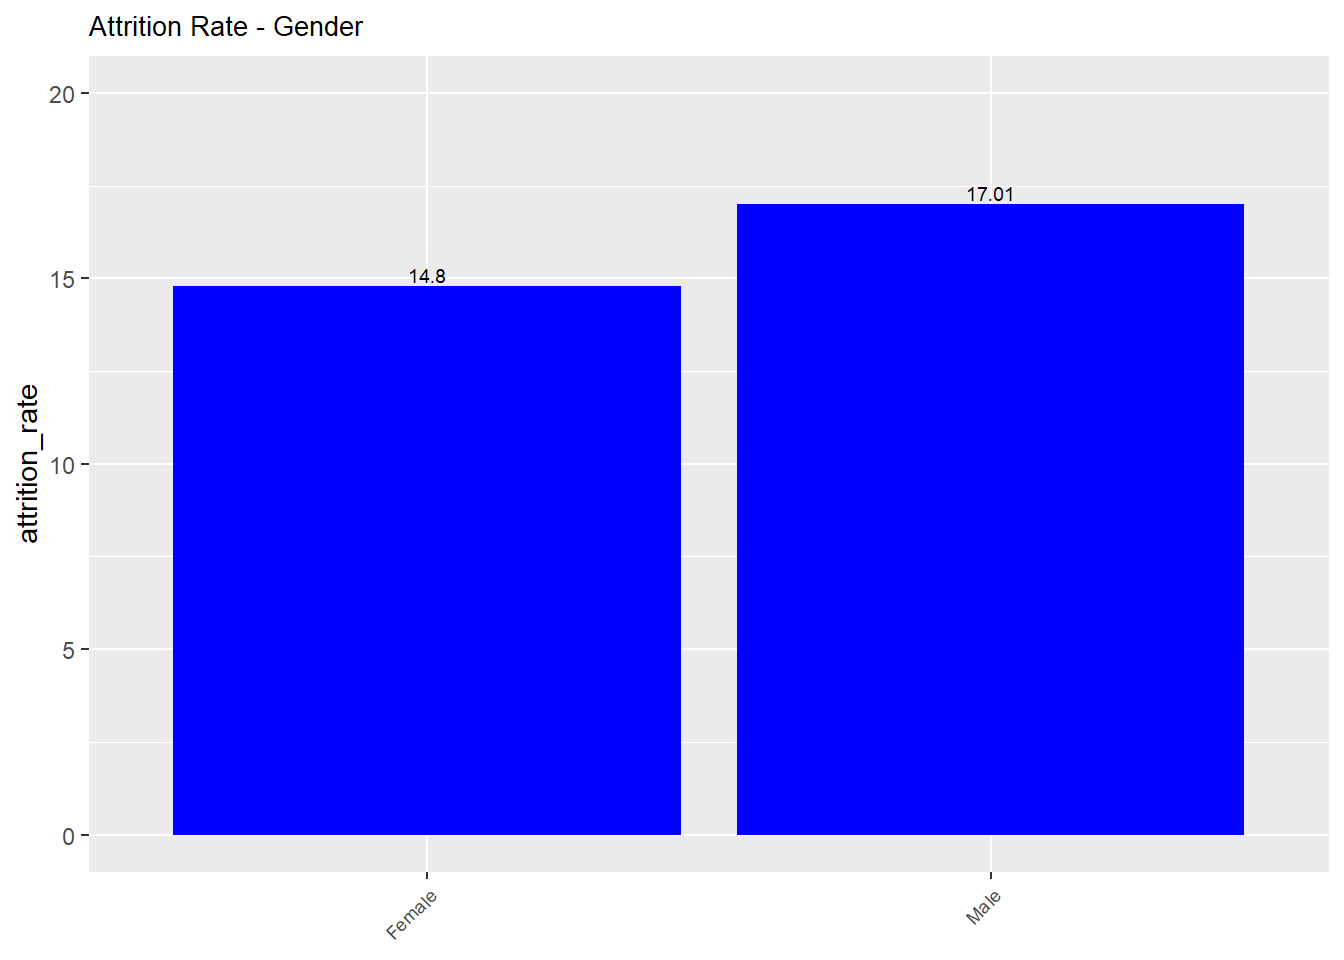
\includegraphics{DDSAnalytics_Case_Study_files/figure-latex/biv_cat_personal-1.pdf}

\subsubsection{Observations}\label{observations-8}

\begin{itemize}
\tightlist
\item
  Male attrition rate is higher than female attrition rate.
\item
  Attrition rate is approximately 18\% for employees with no college
  education.
\item
  Attrition rate is highest for those employees with backgrounds in HR,
  Marketing or a Technical Degree.
\item
  Attrition rate is highest for single employees
\item
  Attrition rate is highest for employees with low relationship
  satisfaction
\item
  Attrition rate is highest for employees with bad work like balance
\end{itemize}

\subsubsection{Employee Demographics - Work
Environment}\label{employee-demographics---work-environment-3}

\begin{Shaded}
\begin{Highlighting}[]
\CommentTok{#Investigate work environment categorical variables such as Business Travel, Overtime, etc as they relate to attrition}
\CommentTok{#Business Travel}
\NormalTok{p1 =}\StringTok{ }\NormalTok{empDF }\OperatorTok
\StringTok{  }\KeywordTok{group_by}\NormalTok{(BusinessTravel) }\OperatorTok
\StringTok{  }\NormalTok{dplyr}\OperatorTok{::}\KeywordTok{summarise}\NormalTok{(}\DataTypeTok{attrition_rate =} \KeywordTok{round}\NormalTok{((}\KeywordTok{sum}\NormalTok{(}\KeywordTok{if_else}\NormalTok{(Attrition }\OperatorTok{==}\StringTok{ "Yes"}\NormalTok{,}\DecValTok{1}\NormalTok{,}\DecValTok{0}\NormalTok{))}\OperatorTok{/}\KeywordTok{n}\NormalTok{()}\OperatorTok{*}\DecValTok{100}\NormalTok{),}\DecValTok{2}\NormalTok{)) }\OperatorTok
\StringTok{  }\KeywordTok{ggplot}\NormalTok{(}\KeywordTok{aes}\NormalTok{(}\DataTypeTok{x =}\NormalTok{ BusinessTravel, }\DataTypeTok{y =}\NormalTok{ attrition_rate))}\OperatorTok{+}\StringTok{ }\KeywordTok{geom_bar}\NormalTok{(}\DataTypeTok{stat =} \StringTok{'identity'}\NormalTok{,}\DataTypeTok{fill =} \StringTok{"blue"}\NormalTok{) }\OperatorTok{+}\StringTok{ }\KeywordTok{ggtitle}\NormalTok{(}\StringTok{"Attrition Rate - Business Travel"}\NormalTok{) }\OperatorTok{+}\StringTok{ }\KeywordTok{theme}\NormalTok{(}\DataTypeTok{plot.title =} \KeywordTok{element_text}\NormalTok{(}\DataTypeTok{size =}\DecValTok{10}\NormalTok{),}\DataTypeTok{axis.text.x =} \KeywordTok{element_text}\NormalTok{(}\DataTypeTok{size =}\DecValTok{7}\NormalTok{,}\DataTypeTok{angle =} \DecValTok{45}\NormalTok{, }\DataTypeTok{hjust =} \DecValTok{1}\NormalTok{),}\DataTypeTok{axis.title.x=}\KeywordTok{element_blank}\NormalTok{()) }\OperatorTok{+}\KeywordTok{geom_text}\NormalTok{(}\KeywordTok{aes}\NormalTok{(}\DataTypeTok{label=}\NormalTok{attrition_rate), }\DataTypeTok{size =} \FloatTok{2.5}\NormalTok{, }\DataTypeTok{position=}\KeywordTok{position_dodge}\NormalTok{(}\DataTypeTok{width=}\FloatTok{0.2}\NormalTok{), }\DataTypeTok{vjust=}\OperatorTok{-}\FloatTok{0.25}\NormalTok{)}\OperatorTok{+}\StringTok{ }\KeywordTok{scale_y_continuous}\NormalTok{(}\DataTypeTok{limits =} \KeywordTok{c}\NormalTok{(}\DecValTok{0}\NormalTok{, }\DecValTok{30}\NormalTok{))}

\CommentTok{#Environment Satisfaction}
\NormalTok{p2 =}\StringTok{ }\NormalTok{empDF }\OperatorTok
\StringTok{  }\KeywordTok{group_by}\NormalTok{(EnvironmentSatisfaction) }\OperatorTok
\StringTok{  }\NormalTok{dplyr}\OperatorTok{::}\KeywordTok{summarise}\NormalTok{(}\DataTypeTok{attrition_rate =} \KeywordTok{round}\NormalTok{((}\KeywordTok{sum}\NormalTok{(}\KeywordTok{if_else}\NormalTok{(Attrition }\OperatorTok{==}\StringTok{ "Yes"}\NormalTok{,}\DecValTok{1}\NormalTok{,}\DecValTok{0}\NormalTok{))}\OperatorTok{/}\KeywordTok{n}\NormalTok{()}\OperatorTok{*}\DecValTok{100}\NormalTok{),}\DecValTok{2}\NormalTok{)) }\OperatorTok
\StringTok{  }\KeywordTok{ggplot}\NormalTok{(}\KeywordTok{aes}\NormalTok{(}\DataTypeTok{x =}\NormalTok{ EnvironmentSatisfaction, }\DataTypeTok{y =}\NormalTok{ attrition_rate))}\OperatorTok{+}\StringTok{ }\KeywordTok{geom_bar}\NormalTok{(}\DataTypeTok{stat =} \StringTok{'identity'}\NormalTok{,}\DataTypeTok{fill =} \StringTok{"blue"}\NormalTok{) }\OperatorTok{+}\StringTok{ }\KeywordTok{ggtitle}\NormalTok{(}\StringTok{"Attrition Rate - Environment Satisfaction"}\NormalTok{) }\OperatorTok{+}\StringTok{ }\KeywordTok{theme}\NormalTok{(}\DataTypeTok{plot.title =} \KeywordTok{element_text}\NormalTok{(}\DataTypeTok{size =}\DecValTok{10}\NormalTok{),}\DataTypeTok{axis.text.x =} \KeywordTok{element_text}\NormalTok{(}\DataTypeTok{size =}\DecValTok{7}\NormalTok{,}\DataTypeTok{angle =} \DecValTok{45}\NormalTok{, }\DataTypeTok{hjust =} \DecValTok{1}\NormalTok{),}\DataTypeTok{axis.title.x=}\KeywordTok{element_blank}\NormalTok{()) }\OperatorTok{+}\KeywordTok{geom_text}\NormalTok{(}\KeywordTok{aes}\NormalTok{(}\DataTypeTok{label=}\NormalTok{attrition_rate), }\DataTypeTok{size =} \FloatTok{2.5}\NormalTok{, }\DataTypeTok{position=}\KeywordTok{position_dodge}\NormalTok{(}\DataTypeTok{width=}\FloatTok{0.2}\NormalTok{), }\DataTypeTok{vjust=}\OperatorTok{-}\FloatTok{0.25}\NormalTok{)}\OperatorTok{+}\StringTok{ }\KeywordTok{scale_y_continuous}\NormalTok{(}\DataTypeTok{limits =} \KeywordTok{c}\NormalTok{(}\DecValTok{0}\NormalTok{, }\DecValTok{30}\NormalTok{))}

\CommentTok{#Job Involvement}
\NormalTok{p3 =}\StringTok{ }\NormalTok{empDF }\OperatorTok
\StringTok{  }\KeywordTok{group_by}\NormalTok{(JobInvolvement) }\OperatorTok
\StringTok{  }\NormalTok{dplyr}\OperatorTok{::}\KeywordTok{summarise}\NormalTok{(}\DataTypeTok{attrition_rate =} \KeywordTok{round}\NormalTok{((}\KeywordTok{sum}\NormalTok{(}\KeywordTok{if_else}\NormalTok{(Attrition }\OperatorTok{==}\StringTok{ "Yes"}\NormalTok{,}\DecValTok{1}\NormalTok{,}\DecValTok{0}\NormalTok{))}\OperatorTok{/}\KeywordTok{n}\NormalTok{()}\OperatorTok{*}\DecValTok{100}\NormalTok{),}\DecValTok{2}\NormalTok{)) }\OperatorTok
\StringTok{  }\KeywordTok{ggplot}\NormalTok{(}\KeywordTok{aes}\NormalTok{(}\DataTypeTok{x =}\NormalTok{ JobInvolvement, }\DataTypeTok{y =}\NormalTok{ attrition_rate))}\OperatorTok{+}\StringTok{ }\KeywordTok{geom_bar}\NormalTok{(}\DataTypeTok{stat =} \StringTok{'identity'}\NormalTok{,}\DataTypeTok{fill =} \StringTok{"blue"}\NormalTok{) }\OperatorTok{+}\StringTok{ }\KeywordTok{ggtitle}\NormalTok{(}\StringTok{"Attrition Rate - Job Involvement"}\NormalTok{) }\OperatorTok{+}\StringTok{ }\KeywordTok{theme}\NormalTok{(}\DataTypeTok{plot.title =} \KeywordTok{element_text}\NormalTok{(}\DataTypeTok{size =}\DecValTok{10}\NormalTok{),}\DataTypeTok{axis.text.x =} \KeywordTok{element_text}\NormalTok{(}\DataTypeTok{size =}\DecValTok{7}\NormalTok{,}\DataTypeTok{angle =} \DecValTok{45}\NormalTok{, }\DataTypeTok{hjust =} \DecValTok{1}\NormalTok{),}\DataTypeTok{axis.title.x=}\KeywordTok{element_blank}\NormalTok{()) }\OperatorTok{+}\KeywordTok{geom_text}\NormalTok{(}\KeywordTok{aes}\NormalTok{(}\DataTypeTok{label=}\NormalTok{attrition_rate), }\DataTypeTok{size =} \FloatTok{2.5}\NormalTok{, }\DataTypeTok{position=}\KeywordTok{position_dodge}\NormalTok{(}\DataTypeTok{width=}\FloatTok{0.2}\NormalTok{), }\DataTypeTok{vjust=}\OperatorTok{-}\FloatTok{0.25}\NormalTok{)}\OperatorTok{+}\StringTok{ }\KeywordTok{scale_y_continuous}\NormalTok{(}\DataTypeTok{limits =} \KeywordTok{c}\NormalTok{(}\DecValTok{0}\NormalTok{, }\DecValTok{40}\NormalTok{))}

\CommentTok{#Job Satisfaction}
\NormalTok{p4 =}\StringTok{ }\NormalTok{empDF }\OperatorTok
\StringTok{  }\KeywordTok{group_by}\NormalTok{(JobSatisfaction) }\OperatorTok
\StringTok{  }\NormalTok{dplyr}\OperatorTok{::}\KeywordTok{summarise}\NormalTok{(}\DataTypeTok{attrition_rate =} \KeywordTok{round}\NormalTok{((}\KeywordTok{sum}\NormalTok{(}\KeywordTok{if_else}\NormalTok{(Attrition }\OperatorTok{==}\StringTok{ "Yes"}\NormalTok{,}\DecValTok{1}\NormalTok{,}\DecValTok{0}\NormalTok{))}\OperatorTok{/}\KeywordTok{n}\NormalTok{()}\OperatorTok{*}\DecValTok{100}\NormalTok{),}\DecValTok{2}\NormalTok{)) }\OperatorTok
\StringTok{  }\KeywordTok{ggplot}\NormalTok{(}\KeywordTok{aes}\NormalTok{(}\DataTypeTok{x =}\NormalTok{ JobSatisfaction, }\DataTypeTok{y =}\NormalTok{ attrition_rate))}\OperatorTok{+}\StringTok{ }\KeywordTok{geom_bar}\NormalTok{(}\DataTypeTok{stat =} \StringTok{'identity'}\NormalTok{,}\DataTypeTok{fill =} \StringTok{"blue"}\NormalTok{) }\OperatorTok{+}\StringTok{ }\KeywordTok{ggtitle}\NormalTok{(}\StringTok{"Attrition Rate - Job Satisfaction"}\NormalTok{) }\OperatorTok{+}\StringTok{ }\KeywordTok{theme}\NormalTok{(}\DataTypeTok{plot.title =} \KeywordTok{element_text}\NormalTok{(}\DataTypeTok{size =}\DecValTok{10}\NormalTok{),}\DataTypeTok{axis.text.x =} \KeywordTok{element_text}\NormalTok{(}\DataTypeTok{size =}\DecValTok{7}\NormalTok{,}\DataTypeTok{angle =} \DecValTok{45}\NormalTok{, }\DataTypeTok{hjust =} \DecValTok{1}\NormalTok{),}\DataTypeTok{axis.title.x=}\KeywordTok{element_blank}\NormalTok{()) }\OperatorTok{+}\KeywordTok{geom_text}\NormalTok{(}\KeywordTok{aes}\NormalTok{(}\DataTypeTok{label=}\NormalTok{attrition_rate), }\DataTypeTok{size =} \FloatTok{2.5}\NormalTok{, }\DataTypeTok{position=}\KeywordTok{position_dodge}\NormalTok{(}\DataTypeTok{width=}\FloatTok{0.2}\NormalTok{), }\DataTypeTok{vjust=}\OperatorTok{-}\FloatTok{0.25}\NormalTok{)}\OperatorTok{+}\StringTok{ }\KeywordTok{scale_y_continuous}\NormalTok{(}\DataTypeTok{limits =} \KeywordTok{c}\NormalTok{(}\DecValTok{0}\NormalTok{, }\DecValTok{30}\NormalTok{))}

\CommentTok{#Overtime}
\NormalTok{p5 =}\StringTok{ }\NormalTok{empDF }\OperatorTok
\StringTok{  }\KeywordTok{group_by}\NormalTok{(OverTime) }\OperatorTok
\StringTok{  }\NormalTok{dplyr}\OperatorTok{::}\KeywordTok{summarise}\NormalTok{(}\DataTypeTok{attrition_rate =} \KeywordTok{round}\NormalTok{((}\KeywordTok{sum}\NormalTok{(}\KeywordTok{if_else}\NormalTok{(Attrition }\OperatorTok{==}\StringTok{ "Yes"}\NormalTok{,}\DecValTok{1}\NormalTok{,}\DecValTok{0}\NormalTok{))}\OperatorTok{/}\KeywordTok{n}\NormalTok{()}\OperatorTok{*}\DecValTok{100}\NormalTok{),}\DecValTok{2}\NormalTok{)) }\OperatorTok
\StringTok{  }\KeywordTok{ggplot}\NormalTok{(}\KeywordTok{aes}\NormalTok{(}\DataTypeTok{x =}\NormalTok{ OverTime, }\DataTypeTok{y =}\NormalTok{ attrition_rate))}\OperatorTok{+}\StringTok{ }\KeywordTok{geom_bar}\NormalTok{(}\DataTypeTok{stat =} \StringTok{'identity'}\NormalTok{,}\DataTypeTok{fill =} \StringTok{"blue"}\NormalTok{) }\OperatorTok{+}\StringTok{ }\KeywordTok{ggtitle}\NormalTok{(}\StringTok{"Attrition Rate - Over Time"}\NormalTok{) }\OperatorTok{+}\StringTok{ }\KeywordTok{theme}\NormalTok{(}\DataTypeTok{plot.title =} \KeywordTok{element_text}\NormalTok{(}\DataTypeTok{size =}\DecValTok{10}\NormalTok{),}\DataTypeTok{axis.text.x =} \KeywordTok{element_text}\NormalTok{(}\DataTypeTok{size =}\DecValTok{7}\NormalTok{,}\DataTypeTok{angle =} \DecValTok{45}\NormalTok{, }\DataTypeTok{hjust =} \DecValTok{1}\NormalTok{),}\DataTypeTok{axis.title.x=}\KeywordTok{element_blank}\NormalTok{()) }\OperatorTok{+}\KeywordTok{geom_text}\NormalTok{(}\KeywordTok{aes}\NormalTok{(}\DataTypeTok{label=}\NormalTok{attrition_rate), }\DataTypeTok{size =} \FloatTok{2.5}\NormalTok{, }\DataTypeTok{position=}\KeywordTok{position_dodge}\NormalTok{(}\DataTypeTok{width=}\FloatTok{0.2}\NormalTok{), }\DataTypeTok{vjust=}\OperatorTok{-}\FloatTok{0.25}\NormalTok{)}\OperatorTok{+}\StringTok{ }\KeywordTok{scale_y_continuous}\NormalTok{(}\DataTypeTok{limits =} \KeywordTok{c}\NormalTok{(}\DecValTok{0}\NormalTok{, }\DecValTok{35}\NormalTok{))}

\CommentTok{#Performance Rating}
\NormalTok{p6 =}\StringTok{ }\NormalTok{empDF }\OperatorTok
\StringTok{  }\KeywordTok{group_by}\NormalTok{(PerformanceRating) }\OperatorTok
\StringTok{  }\NormalTok{dplyr}\OperatorTok{::}\KeywordTok{summarise}\NormalTok{(}\DataTypeTok{attrition_rate =} \KeywordTok{round}\NormalTok{((}\KeywordTok{sum}\NormalTok{(}\KeywordTok{if_else}\NormalTok{(Attrition }\OperatorTok{==}\StringTok{ "Yes"}\NormalTok{,}\DecValTok{1}\NormalTok{,}\DecValTok{0}\NormalTok{))}\OperatorTok{/}\KeywordTok{n}\NormalTok{()}\OperatorTok{*}\DecValTok{100}\NormalTok{),}\DecValTok{2}\NormalTok{)) }\OperatorTok
\StringTok{  }\KeywordTok{ggplot}\NormalTok{(}\KeywordTok{aes}\NormalTok{(}\DataTypeTok{x =} \KeywordTok{as.factor}\NormalTok{(PerformanceRating), }\DataTypeTok{y =}\NormalTok{ attrition_rate))}\OperatorTok{+}\StringTok{ }\KeywordTok{geom_bar}\NormalTok{(}\DataTypeTok{stat =} \StringTok{'identity'}\NormalTok{,}\DataTypeTok{fill =} \StringTok{"blue"}\NormalTok{) }\OperatorTok{+}\StringTok{ }\KeywordTok{ggtitle}\NormalTok{(}\StringTok{"Attrition Rate - Performance Rating"}\NormalTok{) }\OperatorTok{+}\StringTok{ }\KeywordTok{theme}\NormalTok{(}\DataTypeTok{plot.title =} \KeywordTok{element_text}\NormalTok{(}\DataTypeTok{size =}\DecValTok{10}\NormalTok{),}\DataTypeTok{axis.text.x =} \KeywordTok{element_text}\NormalTok{(}\DataTypeTok{size =}\DecValTok{7}\NormalTok{,}\DataTypeTok{angle =} \DecValTok{45}\NormalTok{, }\DataTypeTok{hjust =} \DecValTok{1}\NormalTok{),}\DataTypeTok{axis.title.x=}\KeywordTok{element_blank}\NormalTok{()) }\OperatorTok{+}\KeywordTok{geom_text}\NormalTok{(}\KeywordTok{aes}\NormalTok{(}\DataTypeTok{label=}\NormalTok{attrition_rate), }\DataTypeTok{size =} \FloatTok{2.5}\NormalTok{, }\DataTypeTok{position=}\KeywordTok{position_dodge}\NormalTok{(}\DataTypeTok{width=}\FloatTok{0.2}\NormalTok{), }\DataTypeTok{vjust=}\OperatorTok{-}\FloatTok{0.25}\NormalTok{)}\OperatorTok{+}\StringTok{ }\KeywordTok{scale_y_continuous}\NormalTok{(}\DataTypeTok{limits =} \KeywordTok{c}\NormalTok{(}\DecValTok{0}\NormalTok{, }\DecValTok{20}\NormalTok{))}

\CommentTok{#Department}
\NormalTok{p7 =}\StringTok{ }\NormalTok{empDF }\OperatorTok
\StringTok{  }\KeywordTok{group_by}\NormalTok{(Department) }\OperatorTok
\StringTok{  }\NormalTok{dplyr}\OperatorTok{::}\KeywordTok{summarise}\NormalTok{(}\DataTypeTok{attrition_rate =} \KeywordTok{round}\NormalTok{((}\KeywordTok{sum}\NormalTok{(}\KeywordTok{if_else}\NormalTok{(Attrition }\OperatorTok{==}\StringTok{ "Yes"}\NormalTok{,}\DecValTok{1}\NormalTok{,}\DecValTok{0}\NormalTok{))}\OperatorTok{/}\KeywordTok{n}\NormalTok{()}\OperatorTok{*}\DecValTok{100}\NormalTok{),}\DecValTok{2}\NormalTok{)) }\OperatorTok
\StringTok{  }\KeywordTok{ggplot}\NormalTok{(}\KeywordTok{aes}\NormalTok{(}\DataTypeTok{x =}\NormalTok{ Department, }\DataTypeTok{y =}\NormalTok{ attrition_rate))}\OperatorTok{+}\StringTok{ }\KeywordTok{geom_bar}\NormalTok{(}\DataTypeTok{stat =} \StringTok{'identity'}\NormalTok{,}\DataTypeTok{fill =} \StringTok{"blue"}\NormalTok{) }\OperatorTok{+}\StringTok{ }\KeywordTok{ggtitle}\NormalTok{(}\StringTok{"Attrition Rate - Department"}\NormalTok{) }\OperatorTok{+}\StringTok{ }\KeywordTok{theme}\NormalTok{(}\DataTypeTok{plot.title =} \KeywordTok{element_text}\NormalTok{(}\DataTypeTok{size =}\DecValTok{10}\NormalTok{),}\DataTypeTok{axis.text.x =} \KeywordTok{element_text}\NormalTok{(}\DataTypeTok{size =}\DecValTok{7}\NormalTok{,}\DataTypeTok{angle =} \DecValTok{45}\NormalTok{, }\DataTypeTok{hjust =} \DecValTok{1}\NormalTok{),}\DataTypeTok{axis.title.x=}\KeywordTok{element_blank}\NormalTok{()) }\OperatorTok{+}\KeywordTok{geom_text}\NormalTok{(}\KeywordTok{aes}\NormalTok{(}\DataTypeTok{label=}\NormalTok{attrition_rate), }\DataTypeTok{size =} \FloatTok{2.5}\NormalTok{, }\DataTypeTok{position=}\KeywordTok{position_dodge}\NormalTok{(}\DataTypeTok{width=}\FloatTok{0.2}\NormalTok{), }\DataTypeTok{vjust=}\OperatorTok{-}\FloatTok{0.25}\NormalTok{)}

\CommentTok{#Job Role}
\NormalTok{p8 =}\StringTok{ }\NormalTok{empDF }\OperatorTok
\StringTok{  }\KeywordTok{group_by}\NormalTok{(JobRole) }\OperatorTok
\StringTok{  }\NormalTok{dplyr}\OperatorTok{::}\KeywordTok{summarise}\NormalTok{(}\DataTypeTok{attrition_rate =} \KeywordTok{round}\NormalTok{((}\KeywordTok{sum}\NormalTok{(}\KeywordTok{if_else}\NormalTok{(Attrition }\OperatorTok{==}\StringTok{ "Yes"}\NormalTok{,}\DecValTok{1}\NormalTok{,}\DecValTok{0}\NormalTok{))}\OperatorTok{/}\KeywordTok{n}\NormalTok{()}\OperatorTok{*}\DecValTok{100}\NormalTok{),}\DecValTok{2}\NormalTok{)) }\OperatorTok
\StringTok{  }\KeywordTok{ggplot}\NormalTok{(}\KeywordTok{aes}\NormalTok{(}\DataTypeTok{x =}\NormalTok{ JobRole, }\DataTypeTok{y =}\NormalTok{ attrition_rate))}\OperatorTok{+}\StringTok{ }\KeywordTok{geom_bar}\NormalTok{(}\DataTypeTok{stat =} \StringTok{'identity'}\NormalTok{,}\DataTypeTok{fill =} \StringTok{"blue"}\NormalTok{) }\OperatorTok{+}\StringTok{ }\KeywordTok{ggtitle}\NormalTok{(}\StringTok{"Attrition Rate - Job Role"}\NormalTok{) }\OperatorTok{+}\StringTok{ }\KeywordTok{theme}\NormalTok{(}\DataTypeTok{plot.title =} \KeywordTok{element_text}\NormalTok{(}\DataTypeTok{size =}\DecValTok{10}\NormalTok{),}\DataTypeTok{axis.text.x =} \KeywordTok{element_text}\NormalTok{(}\DataTypeTok{size =}\DecValTok{7}\NormalTok{,}\DataTypeTok{angle =} \DecValTok{45}\NormalTok{, }\DataTypeTok{hjust =} \DecValTok{1}\NormalTok{),}\DataTypeTok{axis.title.x=}\KeywordTok{element_blank}\NormalTok{()) }\OperatorTok{+}\KeywordTok{geom_text}\NormalTok{(}\KeywordTok{aes}\NormalTok{(}\DataTypeTok{label=}\NormalTok{attrition_rate), }\DataTypeTok{size =} \FloatTok{2.5}\NormalTok{, }\DataTypeTok{position=}\KeywordTok{position_dodge}\NormalTok{(}\DataTypeTok{width=}\FloatTok{0.2}\NormalTok{), }\DataTypeTok{vjust=}\OperatorTok{-}\FloatTok{0.25}\NormalTok{)}

\KeywordTok{ggarrange}\NormalTok{(p1,p2,p3,p4,p5,p6,p7,p8)}
\end{Highlighting}
\end{Shaded}

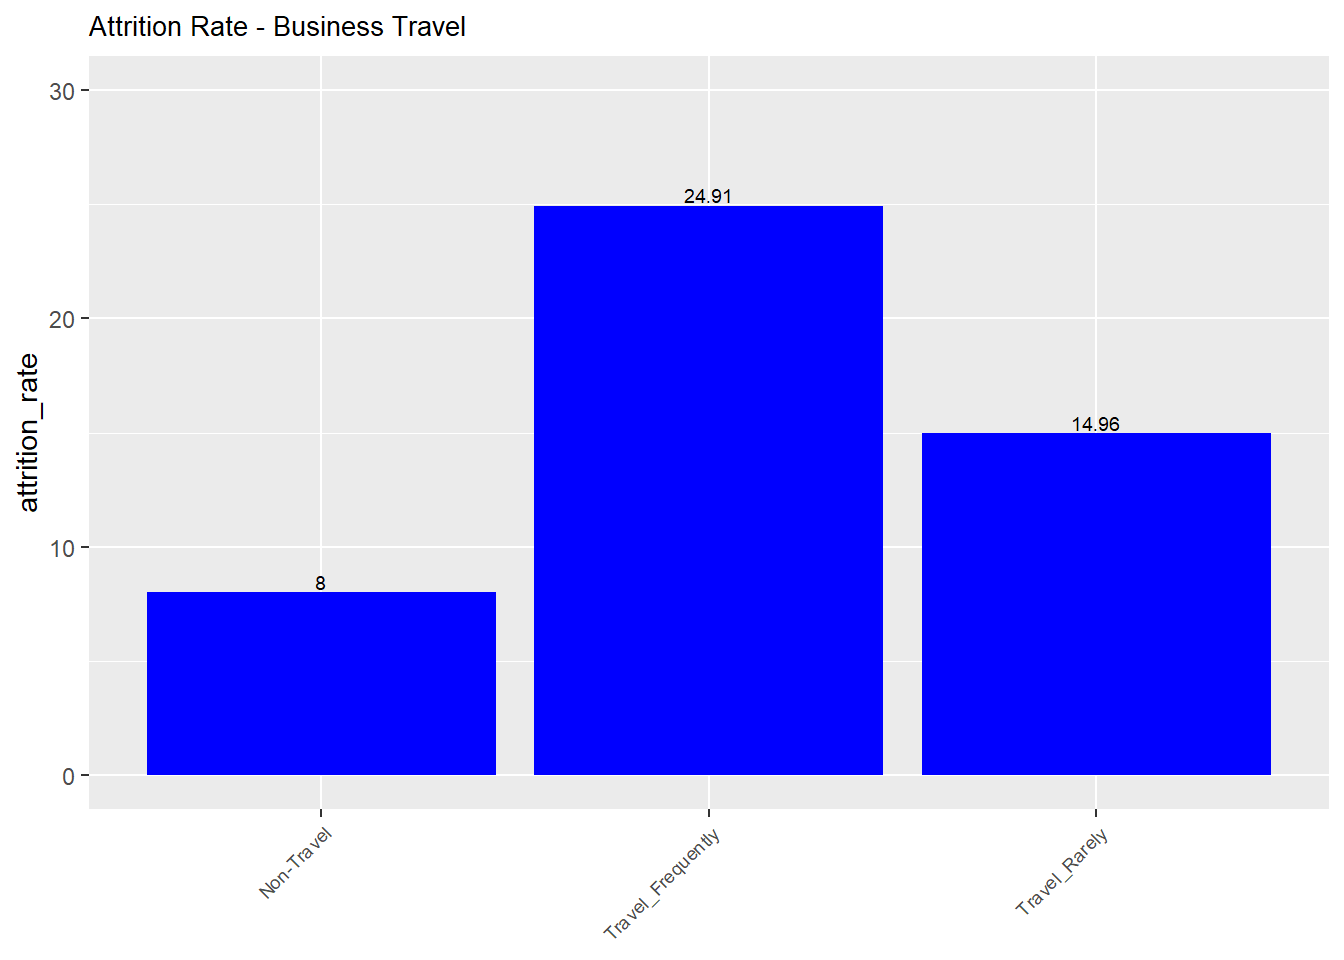
\includegraphics{DDSAnalytics_Case_Study_files/figure-latex/biv_cat_work-1.pdf}

\subsubsection{Observations}\label{observations-9}

\begin{itemize}
\tightlist
\item
  Employees who travel frequently have a higher attrition rate.
\item
  Employees who score environmental satisfaction, job involvement and
  job satisfaction low have higher attrition.
\item
  Employees who work overtime have a higher attrition rate
  (approximately 30\%).
\item
  Employees in the Sales Department have the highest attrition rate at
  20\%.
\item
  Employees who are Sales Representatives have the highest attrition
  rate at 40\%.
\end{itemize}

\begin{center}\rule{0.5\linewidth}{\linethickness}\end{center}

\section{Correlation}\label{correlation}

Now that we've looked at the variables in depth, let's see what
correlations we can find in the data. Break the data up into
non-categorical and categorical variables just as before Credit to David
Josephs - TA for DS6306 for code for the correlator function and
guidance on how best to approach looking at correlation

\subsection{Non-Categorical
Correlations}\label{non-categorical-correlations}

For Non-Categorical (numeric) variables we'll use a heatmap with
correlation coefficients

\begin{Shaded}
\begin{Highlighting}[]
\CommentTok{#Credit to David Joesphs for the function to create the correlation plot.}
\NormalTok{correlator  <-}\StringTok{  }\ControlFlowTok{function}\NormalTok{(df, title)\{}

\NormalTok{    df }\OperatorTok

\StringTok{        }\KeywordTok{keep}\NormalTok{(is.numeric) }\OperatorTok

\StringTok{        }\NormalTok{tidyr}\OperatorTok{::}\KeywordTok{drop_na}\NormalTok{() }\OperatorTok

\StringTok{        }\NormalTok{cor }\OperatorTok

\StringTok{        }\KeywordTok{corrplot}\NormalTok{( }\DataTypeTok{addCoef.col =} \StringTok{"white"}\NormalTok{, }\DataTypeTok{number.digits =} \DecValTok{2}\NormalTok{,}

             \DataTypeTok{number.cex =} \FloatTok{0.5}\NormalTok{, }\DataTypeTok{method=}\StringTok{"square"}\NormalTok{,}

             \DataTypeTok{order=}\StringTok{"hclust"}\NormalTok{, }\DataTypeTok{title=}\NormalTok{title,}

             \DataTypeTok{tl.srt=}\DecValTok{45}\NormalTok{, }\DataTypeTok{tl.cex =} \FloatTok{0.8}\NormalTok{, }\DataTypeTok{mar=}\KeywordTok{c}\NormalTok{(}\DecValTok{0}\NormalTok{,}\DecValTok{0}\NormalTok{,}\DecValTok{1}\NormalTok{,}\DecValTok{0}\NormalTok{))}

\NormalTok{\}}


\KeywordTok{correlator}\NormalTok{(empDF, }\StringTok{"Non-Categorical Variable Heatmap"}\NormalTok{)}
\end{Highlighting}
\end{Shaded}

\includegraphics{DDSAnalytics_Case_Study_files/figure-latex/non_cat_corr-1.pdf}

\subsection{Categorical Correlations}\label{categorical-correlations}

For categorical variables we'll look at boxplots and violin plots

\begin{center}\rule{0.5\linewidth}{\linethickness}\end{center}

\section{Conclusion}\label{conclusion}

From the analysis above we can see that the following variables may have
an influence on attrition:

\begin{itemize}
\tightlist
\item
  Department
\item
  Job Role
\item
  Level of Education
\item
  Amount of Travel
\item
  Amount of Overtime
\item
  Employees with low satisfaction scores in Job Satisfaction, Job
  Engagement and Environmental conditions may also need to be taken into
  account.
\end{itemize}


\end{document}
